\documentclass[a4paper,10pt]{article}

% The following packages can be found on http:\\www.ctan.org
\usepackage{graphicx} % for pdf, bitmapped graphics files
\usepackage{caption}
\usepackage{subcaption}

\graphicspath{{../}}
%\usepackage{epstopdf} % for postscript graphics files
\usepackage{amsmath} % assumes amsmath package installed
\usepackage{amssymb}  % assumes amsmath package installed
\usepackage[caption=false,font=footnotesize]{subfig}
%\usepackage{fixltx2e}
\usepackage{float}

\usepackage[ruled]{algorithm2e}
\usepackage{comment}
\usepackage{color}

\usepackage{hyperref}
\usepackage[hyphenbreaks]{breakurl}

\usepackage{breakcites}


\title{Parameters of the PIV Technique for Deformations Analysis to Static Bending Tests}

\author{Rodrigo Allan Pereira,Fernando Pujaico Rivera,\\%
	Francisco Carlos Gomes,Roberto Alves Braga Junior%
%	\thanks{rodrigo.apereira@deg.ufla.br, fernando.pujaico.rivera@gmail.com,\\%
%		fcgomes@deg.ufla.br,robertobraga@deg.ufla.br}%
}


\begin{document}

\maketitle

%\tableofcontents

\begin{abstract}
The use of particle image velocimetry ($PIV$) technique for flow measurement
in liquid and gaseous materials and in solid deformations 
is an option over conventionally used techniques. This technique, for example, 
can be used in measurements and monitoring of structural parts under load 
with the advantage to be applied in field. However,
$PIV$ technique requires an adequate choice of all parameters to obtain accurate and reliable results. 
The objective of this study is 
the detailed analysis of window size, step size, search size, threshold and 
marker patterns, and their influence  on 
the final result. The study was carried out using test samples of Eucalyptus 
grandis wood subjected to static bending test in a universal testing machine. 
The application of the $PIV$ technique occurred simultaneously to the static 
bending tests. Dial indicators were placed in three regions of the test samples 
for comparison of the deformation values ​​obtained by the two techniques. The 
results showed that the adequate choice of the parameters of  $PIV$ technique 
contributed directly to the non-existence of false positives, increasing its 
precision and reliability.
%\textcolor{red}{It was concluded through this study that the $PIV$
%technique is a tool for measuring deformations with precision similar to 
%conventional test techniques, from the definition and choice of parameters 
%as established in the theoretical models}.
\end{abstract}

\section{INTRODUCTION}
The measurements of deformations in solid surfaces, mainly in structures used in the 
construction industry are of high complexity and demand expensive equipment. This topic is 
currently the object of research with the goal to improve the used techniques, to reduce the 
cost of testing, to promote fast and accurate measurement and to create new testing 
methodologies.%\textcolor{red}{Falta referencia}

The known methodologies may be divided into destructive and non-destructive approaches.
The first one deals with the tests that use the direct contact with the material under 
study, as it happens in the tests executed in Universal Testing Machines ($UTM$). 
Nondestructive testing techniques are those that use physical principles to infer the properties and 
behavior of materials \cite{Pereira2017}. 

The conventional analysis \cite{GOUVEA} 
presents drawbacks such as a high time consuming and number of samples required,
and consequently a high cost of operation. Thus, 
the increase of the use of non-destructive testing techniques is due to the reliability of obtained 
results, with quicker tests  that it does not harm  analyzed materials \cite{DEPAULA}.

Among the non-destructive techniques, optical techniques have become more popular 
in the field of displacement measurement  and deformation in solid bodies. The Particle 
Image Velocimetry ($PIV$) technique is an optical technique with great potential to measure 
displacements and trajectories of particles in a determined body or environment \cite{Pereira2017}.

\begin{sloppypar}
The $PIV$ technique was originally developed in the field of fluids and gases, with 
several applications in this field of study \cite{BANGALEE,XU}. 
Recently, some authors have studied the application of this methodology in solid materials to 
verify deformations and to find the mechanical properties \cite{BRAGAJUNIOR,MAGALHAES,PEREIRA,SOUZA}.
\end{sloppypar}

The main parameter for the execution of the $PIV$ technique is the type of pattern used 
and its distribution on the surface of the sample. The size of the square region of analysis,
 the distance that the algorithm should search a given region of 
analysis from a pre-established point, the search step and the degree of similarity 
between regions of analysis are also important parameters.

This work aims to evaluate the parameters related to the implementation of the $PIV$ 
technique such as the best type of pattern along with its distribution and randomness on the 
surface of the objects under study. In the same way, the parameters directly related to the $PIV$ 
algorithm are studied. These parameters 
are of fundamental importance to the measurement values discriminated by the $PIV$ technique 
to be as accurate as the values obtained by the conventional techniques of test and measurement.

The first section is the introduction and have the basic theory to understand the
$PIV$ analysis, additionally are defined some $PIV$  parameters that will be analyzed.
The second section shows the system setup to the analysis
of the effect of $PIV$ parameters in the $PIV$ procedure.
In the third section is showed the criteria for the selection the $PIV$
parameters. 
%%%%%%
The fourth section show the numerical results of tests presented 
in the second section.
%%%%%%
The fifth section  present the conclusion of article and some considerations.
The last section is a appendix and present the description of used algorithms.
\subsection{Theory}
\subsubsection{Pearson Correlation Coefficient}
The Pearson Correlation Coefficient ($PCC$) \cite{Pearson} measures the correlation degree between two
signals $X$ and $Y$, with $N$ samples denoted by $X_i$ and $Y_i$ respectively.
\begin{equation}
 \rho(X,Y)=\frac{\sum\limits_{i=1}^{N} (X_i-\mu_{X})(Y_i-\mu_{Y})}{N~\sigma_{X}~\sigma_{Y}},
\end{equation} 
where $\mu_{X}$, $\sigma_{X}$, $\mu_{Y}$ and $\sigma_{Y}$ are the expected values and 
the standard deviation values of the signals $X$ and $Y$ respectively.

The range value of the coefficient is between $-1 \leq \rho(X,Y) \leq +1$, where a value close
to $+1$ indicates that there is a high correlation level between $X$ and $Y$, 
on the other hand values close to $0$ indicate that there isn't a correlation and 
finally values close to $-1$ indicate that there is a correlation but with opposite sense,
this means, for example, that when a variable grows the another decreases its value proportionally.

\subsubsection{Particle Image Velocimetry}
The Particle Image Velocimetry ($PIV$) is an optical technique designed 
to flow visualization.
This method needs, to be executed, that the flow in study contain particles, in other words, 
visible elements in the flow; thus
pictures of flow movement are taken and the position of particle groups are
identified between images, forming  a velocity flow map with magnitude and direction \cite{piv1}.

To recognize two identical particle groups between two consecutive images,
many methods may be used, the most widely used method in published material is the
$PCC$ method; for this purpose analysis regions are selected in each image
and if the $PCC$ value, calculated over these data, 
exceeds a threshold, the match is declared and the particle groups
are identified, else ways, another analysis region is selected in  one image and the match test
is performed again.

%In this study line also can be found Particle Tracking Velocimetry (PTV)


\subsection{Parameters of PIV}
\label{sec:systemdesc}

\subsubsection{Analysis region}
An analysis region ($AR$), is a rectangular or square
image portion that is selected to analyze particle groups in the image.
Thus, if two regions are selected, they can be compared to each other using the correlation coefficient.


\subsubsection{Window size}
The window size ($WSIZE$) of a square analysis region
has reference to the length in pixels of the side of this region.
An increment in the $WSIZE$ value promotes an increase of the computational cost of 
method, but in counterpart, an increment in the quantity of the signal information
inside the analysis region, and consequently it decreases the probability of having
a false positive in the match of two analysis region in two images.
On the other hand, small $WSIZE$ values, avoid the loss of correlation 
between two matched analysis regions that undergo deformation.

\subsubsection{Threshold value}
The threshold value ($T$) used in the $PIV$ technique, indicates the minimum value
of $PCC$ that is used to detect a match between two analysis regions.
A high threshold value guarantees that the particle groups in matched 
analysis regions are effectively, the same; but it avoids, that two of the same 
analysis regions be matched when these suffer position deformations in its
particles groups.
Moreover, a low threshold value guarantees that the analysis regions 
can be matched after going through considerable  position deformations in 
its particles groups but widens the possibility of having false positives 
in the matched analysis regions.

\subsubsection{Step length}
The step length ($l_0$) is an integer value in pixels, which is used as minimum dislocation unit 
to choose the portion of the image where the analysis region will be selected from.
Thus, if two analysis regions are selected in two different images, if a match
is not declared between these images, one of these images is discarded and
a new analysis region is selected, distant a $l_0$ (horizontal or vertical) next from
discarded analysis region.


\subsubsection{Search length}
In the same context of the ``Step Length'', the search length ($L$) denotes the maximum
distance (horizontal and vertical) in pixels to select a new  analysis region, 
from the original position of the initial analysis region. Hence 
the distance displaced $nl_0, \forall n\in Z^+,$ to choose a new analysis region,
should be fulfill that $nl_0\leq L$.


\section{MATERIALS AND METHODS}
A static bending test of beams in an universal testing machine (brand AROTEC)
with capacity of at least 300kN was done. The tests were conducted with samples
without defects, from  \textit{Eucalyptus Grandis}  wood, with dimensions of
$2.5 \times 2.5 \times41 cm$. The execution of the tests and the preparation 
of the samples were done based on the norm $ASTM$ $D143-94$ 
\cite{AMERICANSOCIETY}.

\subsection{System setup}
\label{subsec:syssetup}
The $PIV$ technique, in the context of parameter analyses in the static bending test of beams,
It is presented in this work as the tracking of a set of $N=3$ analysis
region (selected in an initial picture) through $M$ pictures taken in standard time intervals ($\tau$).
The Fig. \ref{fig:pivwindow} shows the first picture (left side) 
and the last picture (right side). The picture of the left was taken in
the time $t=0$ and It represents the beam in study with 
$N$ square analysis regions of $WSIZE$ pixels of side; this regions are tracked
across a set of $M$ pictures. The path is shown with red squares in the right side of
the same figure.
\begin{figure}[H]
\centering
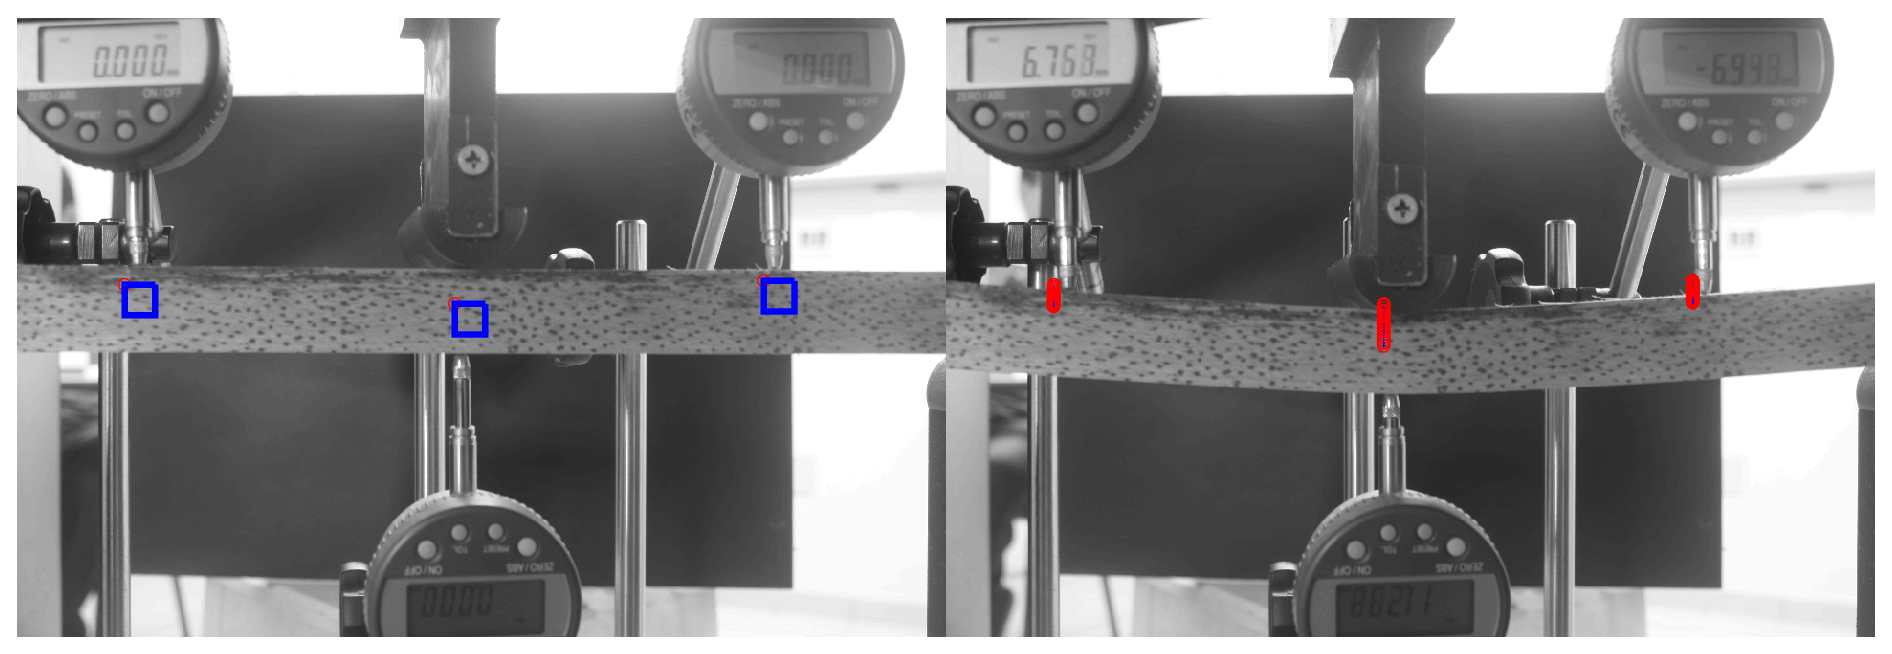
\includegraphics[width=\columnwidth]{numresult1.eps}
\caption{Followed path in a static bending test. 3 dial indicators are used,
two at the ends and one at the center of beam; additionally, in the middle we have a universal testing machine.}
\label{fig:pivwindow}
\end{figure}

Initially the static bending system was compound by a universal testing machine
and  dial indicators to measure the dislocation values of beams,
additionally a digital camera (Canon EOS Rabel T3) was positioned 
to take pictures of the tests. 
A camera was equipped with a lens set to improve
the focusing of the surface of samples; the images were taken through the use of
the remote control to minimize the external interferences in the capture time. 
The detailed arrangement of the instruments in the test can be seen in the Fig. \ref{fig:system1}.
\begin{figure}[H]
\centering
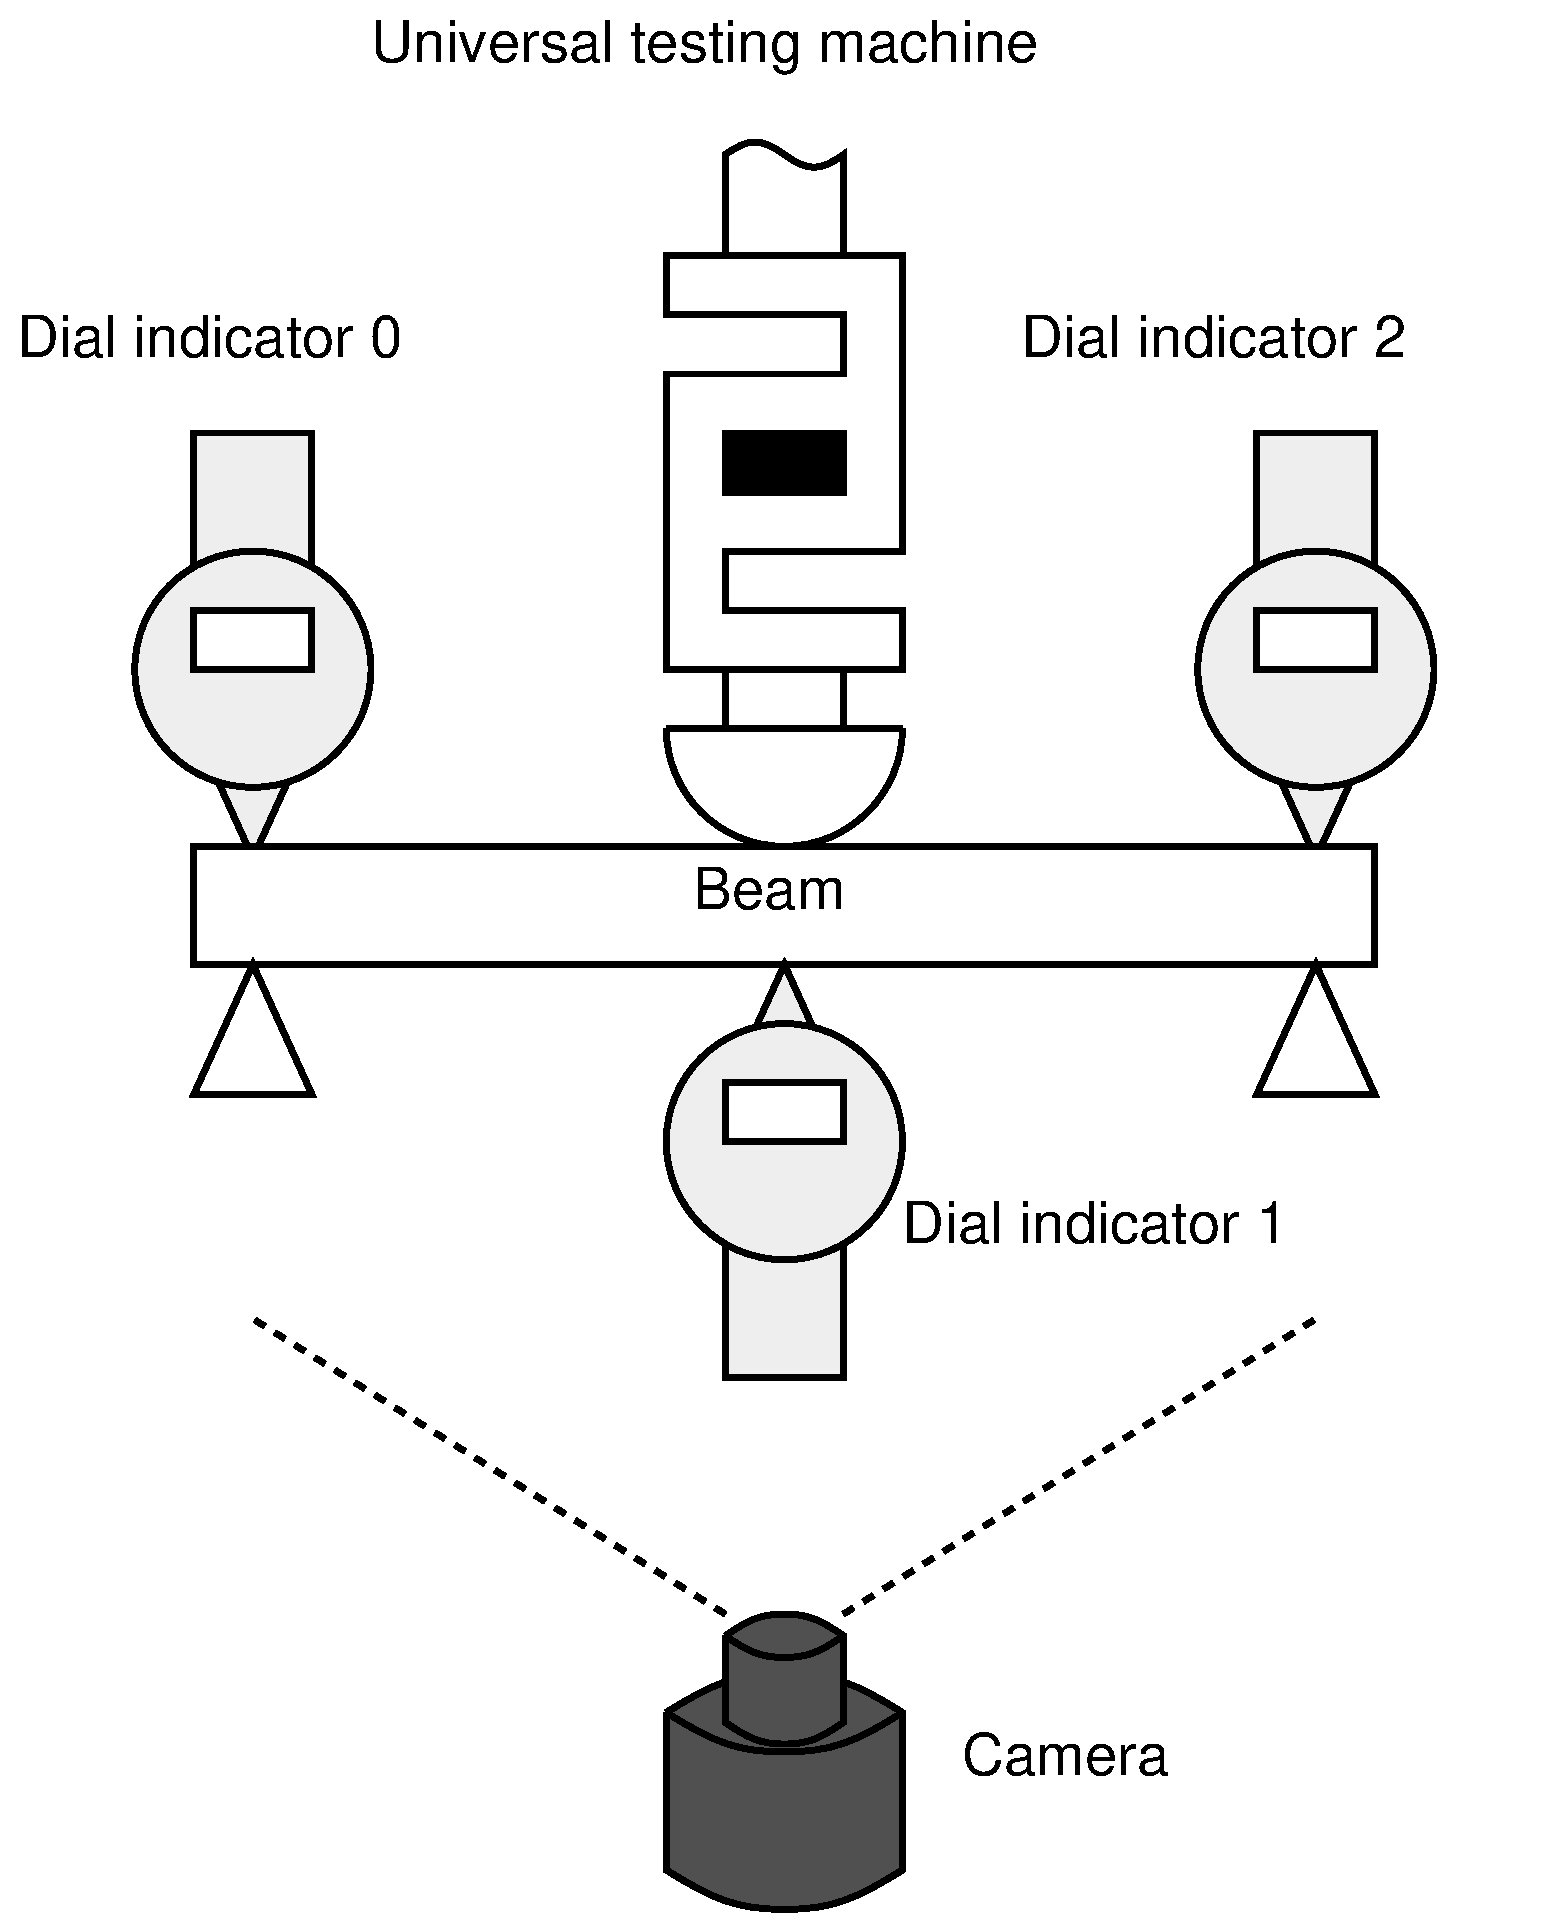
\includegraphics[width=0.45\columnwidth]{Diagrama1.eps}
\caption{System setup description.}
\label{fig:system1}
\end{figure}

In the wood samples, 3 different types of patterns were painted,
the first pattern was painted with spray ($PA$), the second was made marking points, 
with a brush pen, making a regular grid of points with 
$5$ pixels of diameter and $11$ pixels of separation ($PB$), 
and finally in the third were painted
random points of $\sim 5$ pixels of diameter and separation of $\sim 11$ 
pixels  ($PC$), see Fig. \ref{fig:samplesabc}, 
so that the $PIV$ algorithm use these points as particle groups and 
it can track them between consecutive pictures.
\begin{figure}[H]
\centering
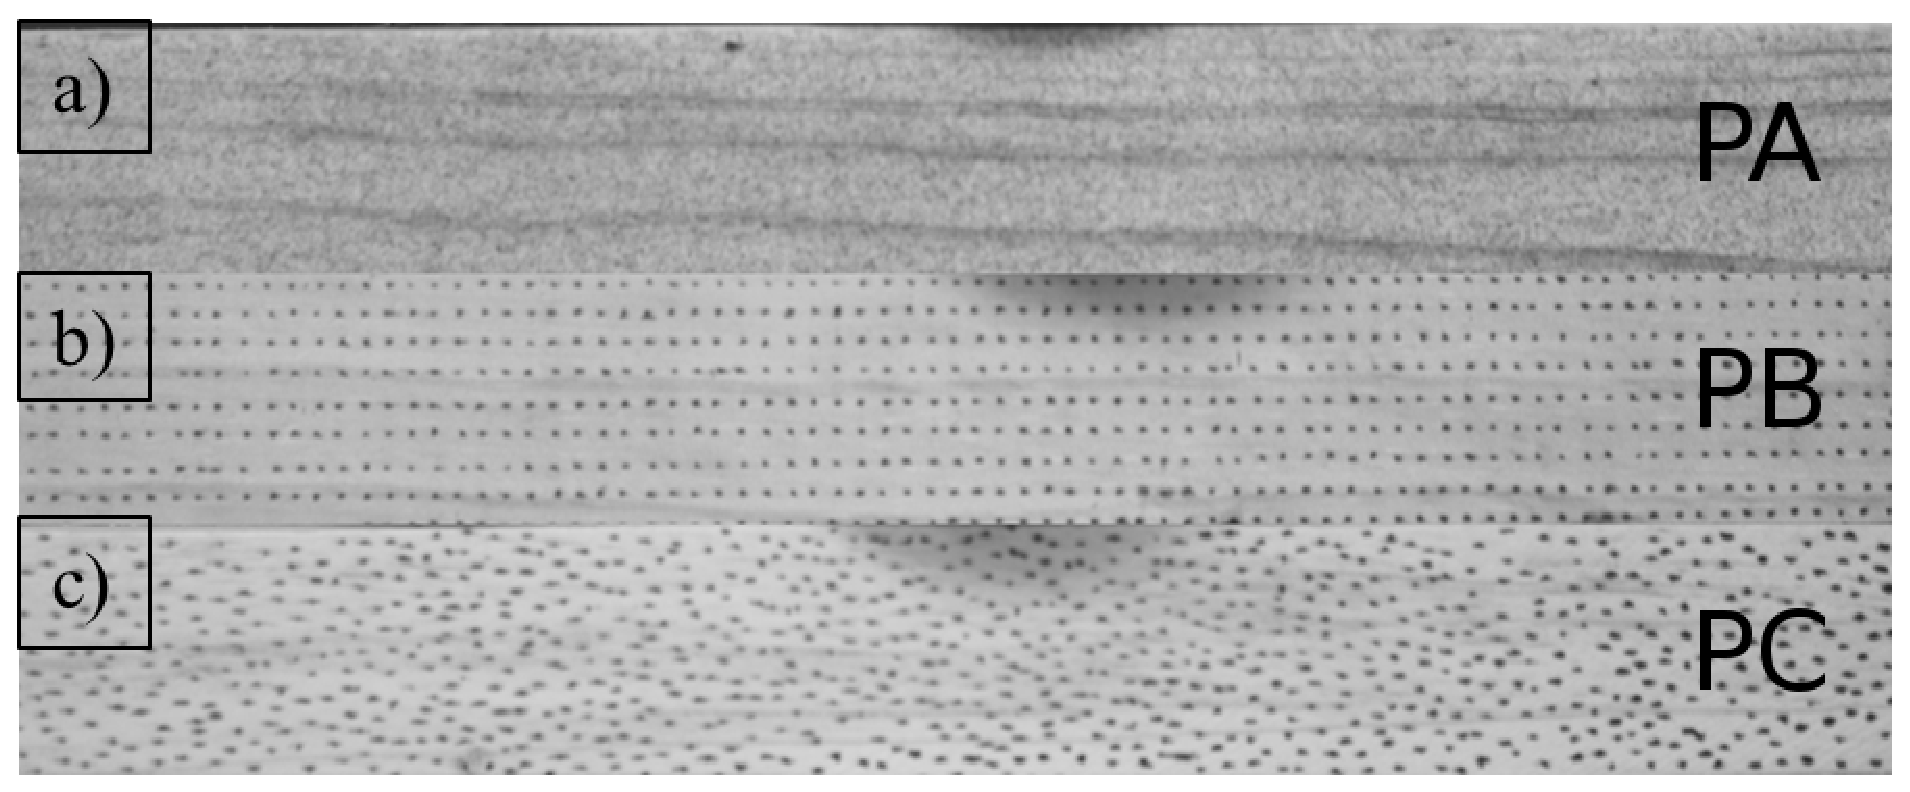
\includegraphics[width=\columnwidth]{abc.eps}
\caption{Surface of the samples with the 3 different patterns. 
$a)$ Black spray paint. $b)$ Points in regular grid with brush pen. $c)$ Random points with brush pen.}
\label{fig:samplesabc}
\end{figure}

It was pre-establishment that, the images would be taken in regular intervals of $\tau=30s$; 
this interval gave us an adequate number of images to execute the procedures. 
The first image was taken at the instant $t=0$ with displacement zero.
after the end of the test, the images were edited to decrease its size in pixels
(change the original image to 8 bit format and decreasing the number of pixels to 25\%);
this procedure is done to  achieve low computational time when
the $PIV$ algorithm is used as described in the appendix, Sec. \ref{sec:algorithm}.


\subsection{Quality tests to patterns and $PIV$ parameters}
\label{sec:qualitytests}
In the next tests we compare 3 types of patterns, over the beams, 
that we call $PA$, $PB$ and $PC$ like presented in 
Fig. \ref{fig:samplesabc}.

\subsubsection{Quality test-1: Displacement test}
The displacement test (test-1) shows the variation of $PCC$ between two analysis regions,
displaced a distance $d$, in a test object with a certain pattern in the surface. 
Thus, being specific,
the test-1 (presented in the Algorithm \ref{alg:displacementtest} of Section \ref{sec:algorithm})
shows the correlations obtained between two square analysis 
regions ($A_{i_0 j_0}$ and $A_{ij}$),
of $WSIZE$ pixels of side, separated by a distance $d=\sqrt{(i-i_0)^2+(j-j_0)^2}$ in pixels.
The initial analysis region is $A_{i_0 j_0}$, and it is chosen in the pixel position $(i_0,j_0)$, 
later this is compared with all others analysis 
regions $A_{ij}$, chosen in the pixel position $(i,j)$, $\forall~i,j \in Z^+|~ 0 \leq |i-i_0| < L$, $~ 0 \leq |j-j_0| < L$.
Thus, for purposes of this analysis we use the patterns $PA$, $PB$ and $PC$ in the side of beam, with
3 different values to $WSIZE$ ($16$, $32$ and $64$).
The next figures show the the result of ``displacement test'' from a pixel position $(i_0,j_0)$.


The Figs. \ref{fig:choosingA16}, \ref{fig:choosingB16} and \ref{fig:choosingC16}
represent the result of displacement test to $WSIZE=16$, 
in the patterns $PA$, $PB$ and $PC$ respectively.
It can be appreciated that in the center of each image exist a maximum of correlation
with value $\rho_0=1.0$, that correspond to the correlation of  $A_{i_0 j_0}$ and $A_{ij}$,
when $i=i_0$ and  $j=j_0$. 
The correlation $\rho_i$ between $A_{i_0 j_0}$ and $A_{ij}$ to $i\neq i_0$ and  $j\neq j_0$;
to the case of pattern $PA$ (Painted with spray) is medium in relation to $\rho_0$
with a maximum value $\rho_i$ of $0.5$, approximately, this condition is acceptable
because if is used a high value of match threshold, then It is 
guaranteed that the region $A_{i_0 j_0}$ only match with itself;
to the case of pattern $PB$ (Grid of dots) the correlation is high in relation to $\rho_0$
with a maximum value $\rho_i$ of $0.9$, approximately, this condition is 
very bad because it can bring false positives in the match of two analysis regions; Finally,
to the case of pattern $PC$ (Aleatory dots) the correlation is medium almost high in relation to $\rho_0$
with a maximum value $\rho_i$ of $0.65$, approximately, this condition is
slightly dangerous because if we use a very low match threshold we can have 
an identification error of the region $A_{i_0 j_0}$.
\begin{figure}[H]
  \centering
  \begin{subfigure}[b]{0.45\textwidth}
    \includegraphics[width=\textwidth]{image_plotA-16.eps}
    \vspace{2pt}
    \caption{Test of pattern $A$.}
    \label{fig:choosingA16}
  \end{subfigure}
  \begin{subfigure}[b]{0.45\textwidth}
    \includegraphics[width=\textwidth]{image_plotB-16.eps}
    \vspace{2pt}
    \caption{Test of pattern $B$.}
    \label{fig:choosingB16}
  \end{subfigure}
  \begin{subfigure}[b]{0.45\textwidth}
    \includegraphics[width=\textwidth]{image_plotC-16.eps}
    \vspace{2pt}
    \caption{Test of pattern $C$.}
    \label{fig:choosingC16}
  \end{subfigure}
  \caption{Displacement test to $WSIZE=16$.}
  \label{fig:choosingAll16}
\end{figure}


The Figs. \ref{fig:choosingA32}, \ref{fig:choosingB32} and \ref{fig:choosingC32}
represent the result of displacement test to $WSIZE=32$, 
in the patterns $PA$, $PB$ and $PC$ respectively. Similarly to the last case,
It can be appreciated that in the center of each image exist a maximum of correlation
with value $\rho_0=1.0$. Thus,
the correlation $\rho_i$ between $A_{i_0 j_0}$ and $A_{ij}$ to $i\neq i_0$ and  $j\neq j_0$;
to the case of pattern $PA$ (Painted with spray) is very low in relation to $\rho_0$
with a maximum value $\rho_i$ of $0.2$, approximately, 
so that the region $A_{i_0 j_0}$ only match with itself;
to the case of pattern $PB$ (Grid of dots) the correlation is medium in relation to $\rho_0$
with a maximum value $\rho_i$ of $0.8$, approximately, this condition is 
very bad because it can bring false positives in the match of two analysis regions; Finally,
to the case of pattern $PC$ (Aleatory dots) the correlation is very low in relation to $\rho_0$
with a maximum value $\rho_i$ of $0.4$, approximately, this condition is acceptable
because if is used a high value of match threshold, then It is 
guaranteed that the region $A_{i_0 j_0}$ only match with itself;
\begin{figure}[H]
  \centering
  \begin{subfigure}[b]{0.45\textwidth}
    \includegraphics[width=\textwidth]{image_plotA-32.eps}
    \vspace{2pt}
    \caption{Test of pattern $A$.}
    \label{fig:choosingA32}
  \end{subfigure}
  \begin{subfigure}[b]{0.45\textwidth}
    \includegraphics[width=\textwidth]{image_plotB-32.eps}
    \vspace{2pt}  
    \caption{Test of pattern $B$.}
    \label{fig:choosingB32}
  \end{subfigure}
  \begin{subfigure}[b]{0.45\textwidth}
    \includegraphics[width=\textwidth]{image_plotC-32.eps}
    \vspace{2pt}
    \caption{Test of pattern $C$.}
    \label{fig:choosingC32}
  \end{subfigure}
  \caption{Displacement test to $WSIZE=32$.}
  \label{fig:choosingAll32}
\end{figure}

The Figs. \ref{fig:choosingA64}, \ref{fig:choosingB64} and \ref{fig:choosingC64}
represent the result of displacement test to $WSIZE=64$, 
in the patterns $PA$, $PB$ and $PC$ respectively. Similarly to the last case,
It can be appreciated that in the center of each image exist a maximum of correlation
with value $\rho_0=1.0$. Thus,
the correlation $\rho_i$ between $A_{i_0 j_0}$ and $A_{ij}$ to $i\neq i_0$ and  $j\neq j_0$;
to the case of pattern $PA$ (Painted with spray) is low in relation to $\rho_0$
with a maximum value $\rho_i$ of $0.3$, approximately, 
so that the region $A_{i_0 j_0}$ only match with itself;
to the case of pattern $PB$ (Grid of dots) the correlation is medium in relation to $\rho_0$
with a maximum value $\rho_i$ of $0.8$, approximately, this condition is 
very bad because it can bring false positives in the match of two analysis regions; Finally,
to the case of pattern $PC$ (Aleatory dots) the correlation is very low in relation to $\rho_0$
with a maximum value $\rho_i$ of $0.2$, approximately, 
so that the region $A_{i_0 j_0}$ only match with itself;
\begin{figure}[H]
\centering
  \begin{subfigure}[b]{0.45\textwidth}
    \includegraphics[width=\textwidth]{image_plotA-64.eps}
    \vspace{2pt}
    \caption{Test of pattern $A$.}
    \label{fig:choosingA64}
  \end{subfigure}
  \begin{subfigure}[b]{0.45\textwidth}
    \includegraphics[width=\textwidth]{image_plotB-64.eps}
    \vspace{2pt}
    \caption{Test of pattern $B$.}
    \label{fig:choosingB64}
  \end{subfigure}
  \begin{subfigure}[b]{0.45\textwidth}
    \includegraphics[width=\textwidth]{image_plotC-64.eps}
    \vspace{2pt}
    \caption{Test of pattern $C$.}
    \label{fig:choosingC64}
  \end{subfigure}
  \caption{Displacement test to $WSIZE=64$.}
  \label{fig:choosingAll64}
\end{figure}

Finally, to a better understanding of the data in the Figs.
\ref{fig:choosingAll16}, \ref{fig:choosingAll32} and \ref{fig:choosingAll64},
they were create the Figs. 
\ref{fig:choosingt16}, \ref{fig:choosingt32} and \ref{fig:choosingt64},
 respectively.
Each new figure represents in a polar diagram around $(i_0,j_0)$, the lost of correlation
of the $3$ different patterns; so that the
distance $d$ in pixels represent a distance to position $(i_0,j_0)$; 
it is important to note in the figures that, if many pixel positions
represent the same distance, then only It is plotted the value with the highest correlation.
Thus, this new figures allow us to intuit, using a two-dimensional graphic,
how can exist false positives in the matching with regions neighboring to the origin.
\begin{figure}[H]
\centering
  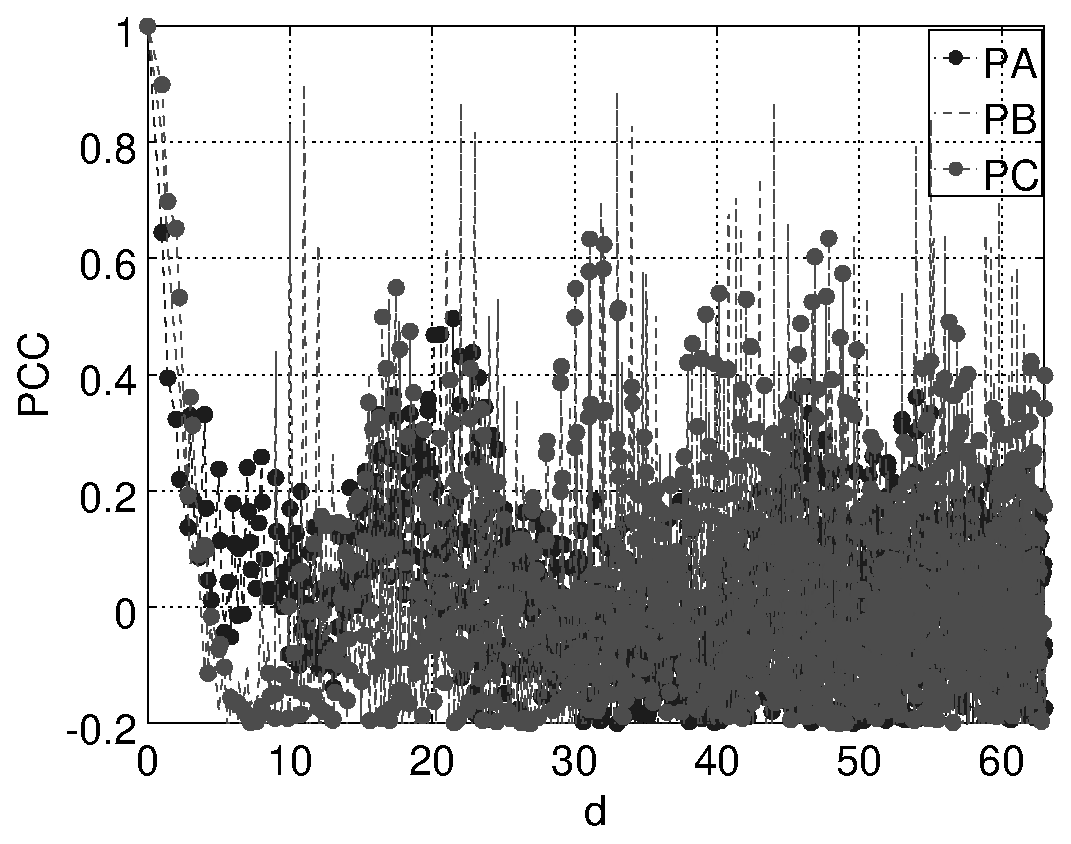
\includegraphics[width=.55\columnwidth]{image_plot-16.eps}
  \caption{Correlation of analysis regions in relation to the distance to $(i_0,j_0)$ to a $WSIZE=16$.}
  \label{fig:choosingt16}
\end{figure}
For example, in the Fig. \ref{fig:choosingt16} to the patterns $PA$, $PB$ and $PC$,
exist a high $PCC$ with analysis regions distant beyond 8 pixels, so that
It is very possible exist a false positive in the identification of a analysis 
region. The worst case is  obtained using the pattern $PB$, that reaches higher values
to $0.8$ in the correlation; the periodicity of $PCC$ value in this pattern
is a consequence of the periodicity of pattern.
\begin{figure}[H]
\centering
  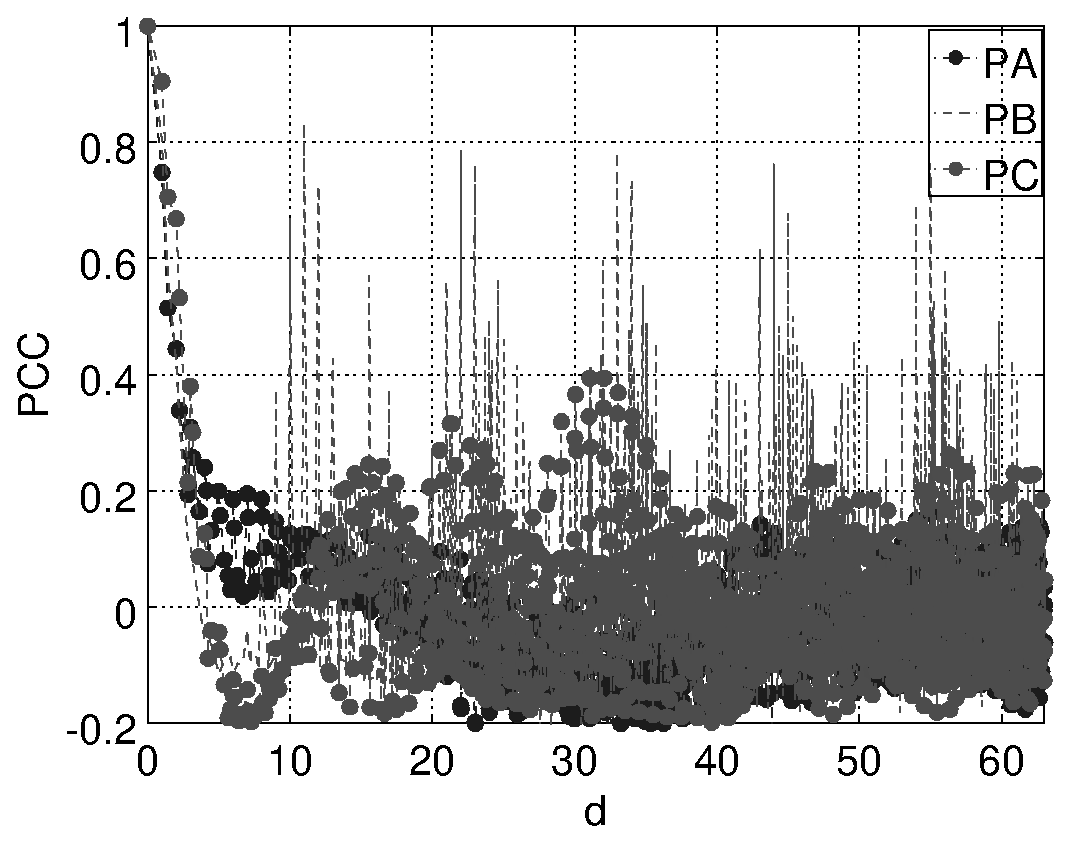
\includegraphics[width=.55\columnwidth]{image_plot-32.eps}
  \caption{Correlation of analysis regions in relation to the distance to $(i_0,j_0)$ to a $WSIZE=32$.}
  \label{fig:choosingt32}
\end{figure}
By other side, in the Fig. \ref{fig:choosingt32}, the $PCC$ value decays irregularly with 
distance in the patterns $PA$ and $PC$, as expected. But the pattern $PB$ still 
a high level of correlation with  peaks located with periodicity.
\begin{figure}[H]
\centering
  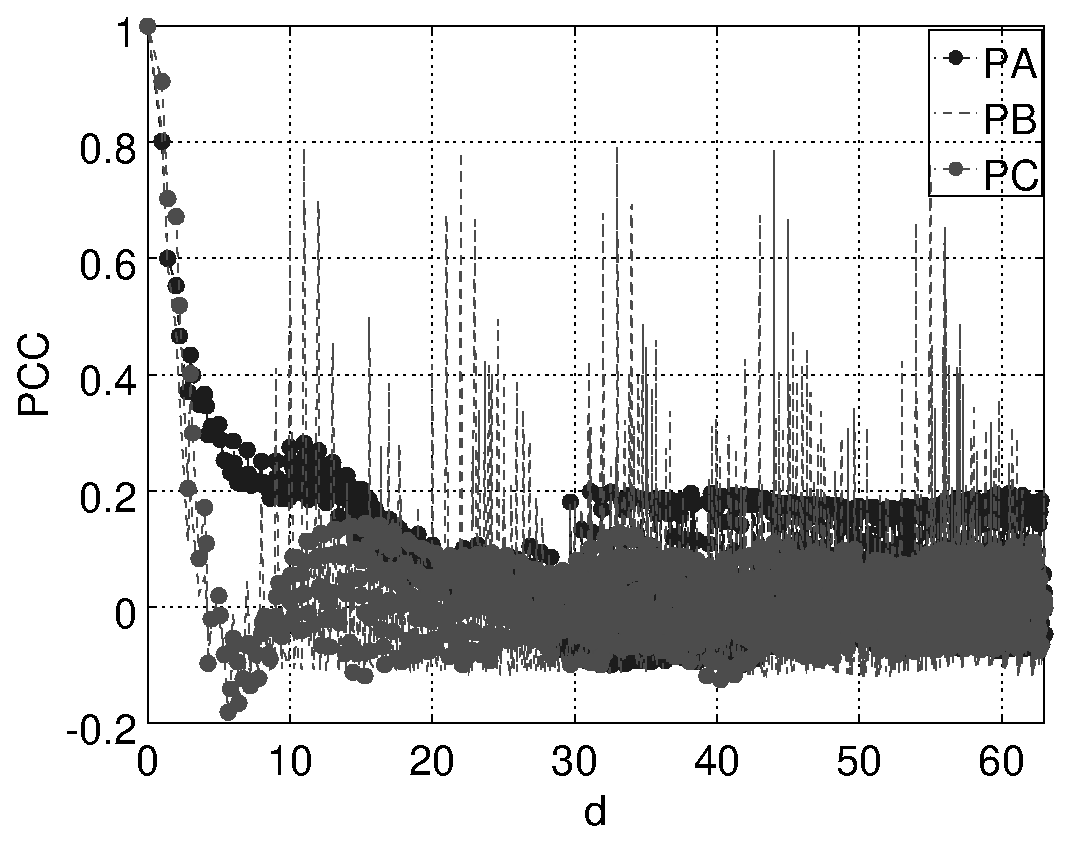
\includegraphics[width=.55\columnwidth]{image_plot-64.eps}
  \caption{Correlation of analysis regions in relation to the distance to $(i_0,j_0)$ to a $WSIZE=64$.}
  \label{fig:choosingt64}
\end{figure}
Finally, in the Fig. \ref{fig:choosingt64}, the $PCC$ value decays monotonously with 
distance in the patterns $PA$ and $PC$. The pattern $PB$ continues to have 
correlation problems.


\subsubsection{Quality test-2: Rotation test}
The test-2 (presented in the Algorithm \ref{alg:rotationtest} of Section \ref{sec:algorithm}) 
shows the correlations between two square analysis regions 
($B_0$ and $B_i$),
of $WSIZE$ pixels of side; so that $B_i$ is a rotated version, an angle $\alpha_i=0.5 i$, 
of analysis region $B_0$, $\forall~i\in Z^+~|~0  \leq  i \leq 23$. 
The purpose of this test is to know the lost of correlation when the body under study
suffers a distortion  that causes a rotation of the analysis region $B_0$.
Thus, the Figs. \ref{fig:choosingr16}, \ref{fig:choosingr32} and \ref{fig:choosingr64}
show the correlation values for two analysis regions rotated until an angle of $\alpha_{max}=11.5^\circ$,
in each figure is shown the behavior to the 3 types of patterns. Being that the Fig. \ref{fig:choosingr16}
use a $WSIZE=16$, the Fig. \ref{fig:choosingr32} a $WSIZE=32$ and the last a $WSIZE=64$.
\begin{figure}[H]
  \centering
  \begin{subfigure}[b]{0.45\textwidth}
    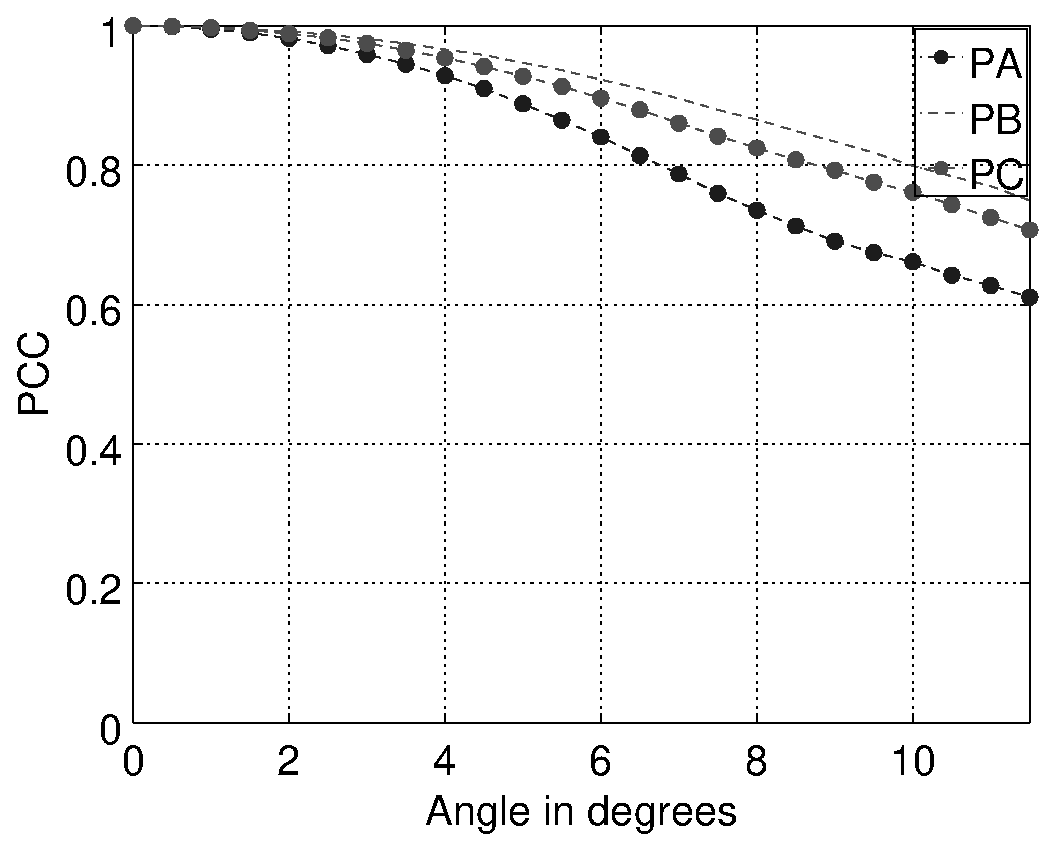
\includegraphics[width=\textwidth]{image_rot_plot-16.eps}
    \vspace{2pt}
    \caption{Rotation test to $WSIZE=16$.}
    \label{fig:choosingr16}
  \end{subfigure}
  \begin{subfigure}[b]{0.45\textwidth}
    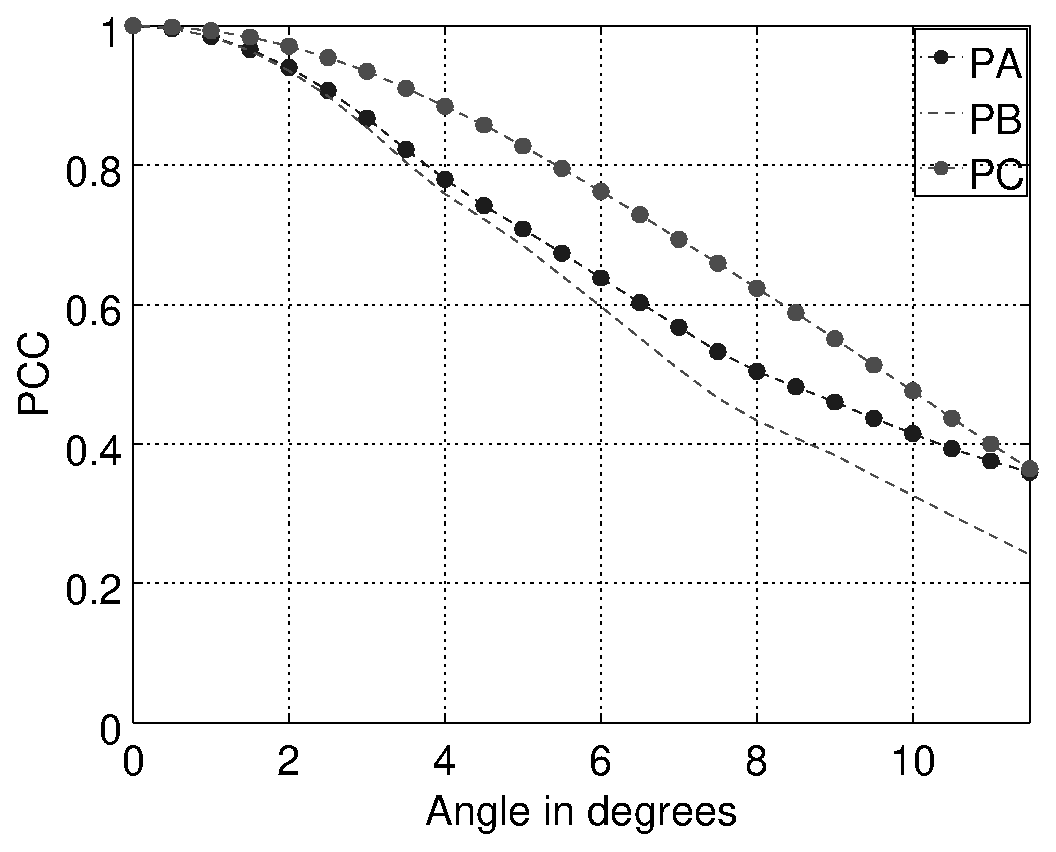
\includegraphics[width=\textwidth]{image_rot_plot-32.eps}
    \vspace{2pt}
    \caption{Rotation test to $WSIZE=32$.}
    \label{fig:choosingr32}
  \end{subfigure}
  \begin{subfigure}[b]{0.45\textwidth}
    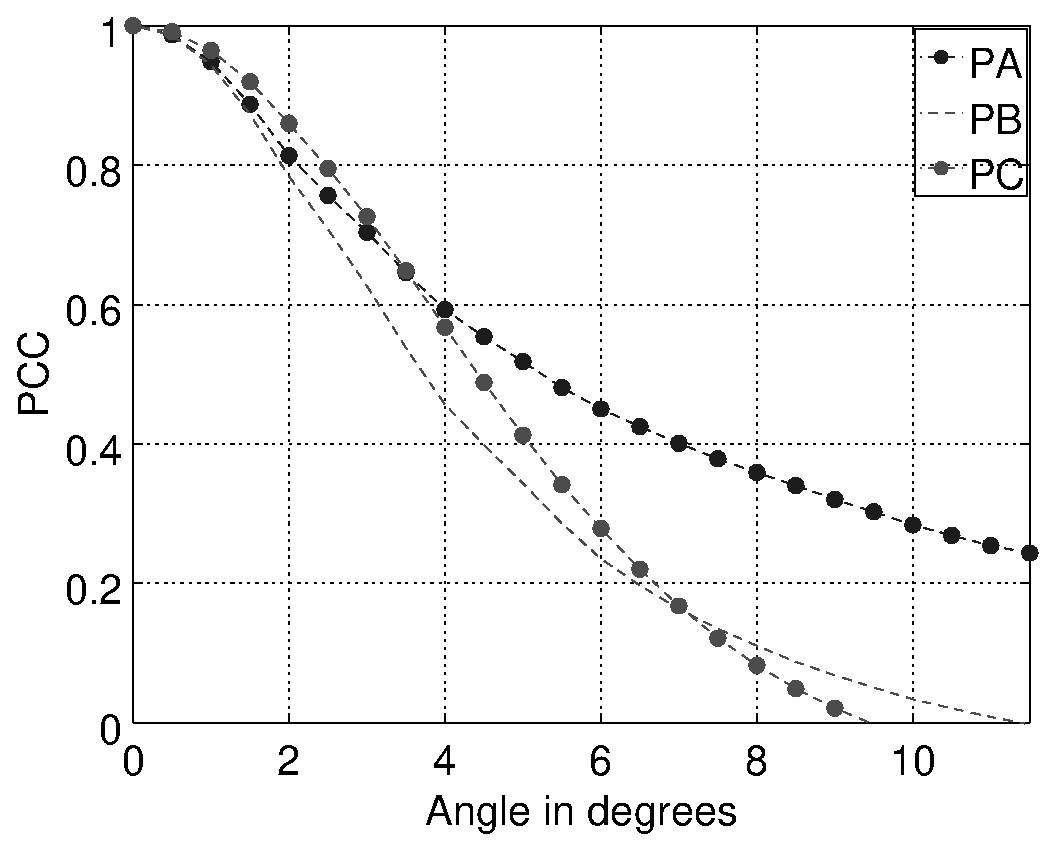
\includegraphics[width=\textwidth]{image_rot_plot-64.eps}
    \vspace{2pt}
    \caption{Rotation test to $WSIZE=64$.}
    \label{fig:choosingr64}
  \end{subfigure}
  \caption{Rotation test to different values of analysis region side $WSIZE$.}
  \label{fig:RotationAll}
\end{figure}

The Fig. \ref{fig:choosingr16} shows a low correlation loss by the 
rotation of a region $B_0$ in all patterns; being that the patterns $PB$ and $PC$ have
the best response to the rotation, holding a $PCC>0.7$ to rotation angles minors that $11.5^\circ$.
This meaning that using a threshold value of $0.7$, the $PIV$ technique in the patterns $PB$ and $PC$
can identify the region $B_0$, even if it has been rotated, up to an angle of $11.5^\circ$;
and the patterns $PA$ to the same threshold only supports a maximum rotation of an angle of $8.25^\circ$.
In a similar way, using a threshold value of $0.7$, in the Fig. \ref{fig:choosingr32},
the patterns $PA$ and $PB$ only support a maximum rotation of an angle of $5.0^\circ$, and
the pattern $PC$ an angle of $7.0^\circ$.
Finally, using the same threshold, in the Fig. \ref{fig:choosingr64},
the patterns $PA$, $PB$ and $PC$ only support a maximum rotation of an angle of $3.0^\circ$, approximately.

In general is evident that, when the value $WSIZE$ grow up, the maximum angle that support the
$PIV$ technique to recognize a rotated region, decreases.




\section{CRITERIA FOR VARIABLE SELECTION}
\label{sec:criteria}
\subsection{Choosing the type of pattern}

In the test-1 we can see the correlation analysis of 3 types of patterns
(see Fig. \ref{fig:samplesabc}). This results can be used to select the best pattern
to use in the  load and break study of beams; for example, following the 
Figs. \ref{fig:choosingt16}, \ref{fig:choosingt32} and \ref{fig:choosingt64},
is easy to see that a periodic pattern as $PB$ has also a periodic behavior
in the $PCC$ value; so that we have that consider values of threshold $T \geq 0.82$ 
in the Figs. \ref{fig:choosingt32} and \ref{fig:choosingt64} and $T \geq 0.90$
in the Fig. \ref{fig:choosingt16}, so that
less values of these threshold have the probability of causing false positives in the recognition of an 
analysis region. Given that, in the pattern $PB$, many positions share correlation values with similar values
for a threshold relatively high like $T=0.75$, we not recommend to use periodic patterns like $PB$.

The patterns $PA$ and $PC$ are random in nature, with the difference
that the pattern points in $PC$ are big  and few, and in the $PA$
are many and small. Following the 
Figs. \ref{fig:choosingt16}, \ref{fig:choosingt32} and \ref{fig:choosingt64},
we can see that the $PCC$ values have a behavior approximately monotone decrescent
when the size of analysis region is greater when compared to the size of points
in the pattern. Thus, the pattern $PA$ and $PC$ have a strange behavior to a $WSIZE=16$;
so that the $T$ value, necessary to have  a false positive is
$T<0.60$ to $PA$ and $PC$; we can see this clearly in the Fig. \ref{fig:choosingt16} 
given that the values of $PCC$ that fulfill this condition only are very close to the origin.
In the same sense to a value $WSIZE = 32$, 
the threshold conditions necessary to have  false positives
are $T<0.2$ and $T<0.4$ to $PA$ and $PC$, respectively; these values of $PCC$ are much lower 
and close to the origin therefore never lead to confusion.
Finally, to a  value $WSIZE = 64$, 
the threshold conditions necessary to have  a false positive 
are $T<0.3$ and $T<0.2$ to $PA$ and $PC$, respectively; 
these values of $PCC$ are lower like the one obtained with $WSIZE = 32$,
therefore these are equally convenient to those obtained with $WSIZE = 32$.
Thus, in the Figs. \ref{fig:choosingt16}, \ref{fig:choosingt32} and \ref{fig:choosingt64},
there is not a clear advantage of $PA$ over $PC$ given that both support analysis regions
of $WSIZE \geq 32$.

In the test-2 we can see the correlation analysis of two rotated analysis regions, 
to the 3 types of patterns seen in the Fig. \ref{fig:samplesabc}.
For a fair comparison, we establish the value $PCC=0.82$ as the analysis line to the
Figs. \ref{fig:choosingr16}, \ref{fig:choosingr32} and \ref{fig:choosingr64}, 
given that we consider that
values lower this given us an error in the recognition of the analysis region.
In the Figs.  \ref{fig:choosingr16} and \ref{fig:choosingr32} there is
a marked difference  to recognize an analysis region in favor to the
pattern $PC$, given that this support a superior rotation angle range. Additionally,
in the Fig. \ref{fig:choosingr64} we observe that there is not a 
significant difference between the angle range  when the patterns
$PA$ and $PC$ are compared.
Here, it is important  to note
that in all cases an analysis region with a very large $WSIZE$,
 when compared to the size of the points in the pattern
 (in this case $WSIZE=64$ ), prevents identifying the rotated analysis region correctly.
 This is expected given that 
the deviation to a distance $d_0$ caused by an angle $\alpha_0$ is less significant that
a deviation to a distance $2d_0$. The effect of the rotation is very important 
in the  load and break study of beams, given that in these tests
there are small angle rotations in regions analyzed between to consecutive images.

Thus, we recommend the use of patterns such as $PC$ (with big dot patterns) 
given that to analysis regions, rotated a small angle,
these hold better the $PCC$ value; and consequently the correlation analysis 
is able to identify better a rotated region. 

\subsection{Choosing the window size}

As can be seen in the Test-1, the value of $WSIZE$
influences the recognition of displaced analysis regions.
Thus, a pattern such as $PC$, with patterns points of 
$5$ pixels of diameter and separation of $11$ pixels,
needs  a $WSIZE > 32$ to avoid false positives in the 
analysis region recognition process using a threshold value relatively 
lower, see Fig \ref{fig:choosingt32};
given that, analysis regions with $WSIZE \leq 32$ results in regions with a few
characteristic details (information) and the probability of
finding a similar region is high.

On the other hand as can be seen in the Test-2, the value of $WSIZE$
also influences the recognition of rotated analysis regions.
So that, for a pattern as $PC$, a $WSIZE=64$ only allows
recognition of analysis regions rotated at most a angle of $2.5^\circ$
(for a threshold of $PCC=0.82$). 
Thus, to a pattern like $PC$ (similar diameter and separation of pattern points), 
we recommend to use  a $32 \leq WSIZE \leq 64$.


\subsection{Choosing the threshold value}

For a pattern as $PC$, the choice of a threshold $T$
depends on the used value for $WSIZE$; for example, in the Fig. 
\ref{fig:choosingt16}, 
where is used a $WSIZE=16$,  
the form of the correlation curve limits the threshold
to a value of $T \geq 0.60$, given that smaller values
cause false positives in the recognition process of analysis regions.
Furthermore in the Fig. \ref{fig:choosingt32}
the correlation curve limits the threshold
to a value of $T \geq 0.40$. In all these cases, the specific used 
threshold value of $PCC$ will chosen
taking into account the chosen step length $l_0$.


\subsection{Choosing the step length}
\label{subsec:steplength}

The first thing to consider is that if we define a step length such
as $l_0$ pixels, the maximum (bi-dimensional) measure error, 
in predicting the displacement of an analysis region between two consecutive images,
will be of $l_0\sqrt{2}/2$ pixels. Thus if the step length is $l_0=1$ pixel, then
the maximum displacement error will be of $0.70711$ pixels; being this the minimum
(desirable) of the maximum displacement error in the technique, and we recommend
the use of image sizes that allow acceptable processing times with a step length of
$l_0=1$ pixel. But if is desired to use other values to the step length,
we should take in consideration other involve variables such as the used threshold.

For example, if we establish the threshold for a value of $PCC=0.67$ in the
test-1, where a $WSIZE=32$ is used
(see Fig. \ref{fig:choosingt32zoom}),
then we observe that, for the pattern $PC$, the error in the displacement prediction before
losing the analysis region in the recognition process, it is of $2$ pixels,
or in others words $l_0\sqrt{2}/2 \leq 2$ pixels.
\begin{figure}[H]
\centering
  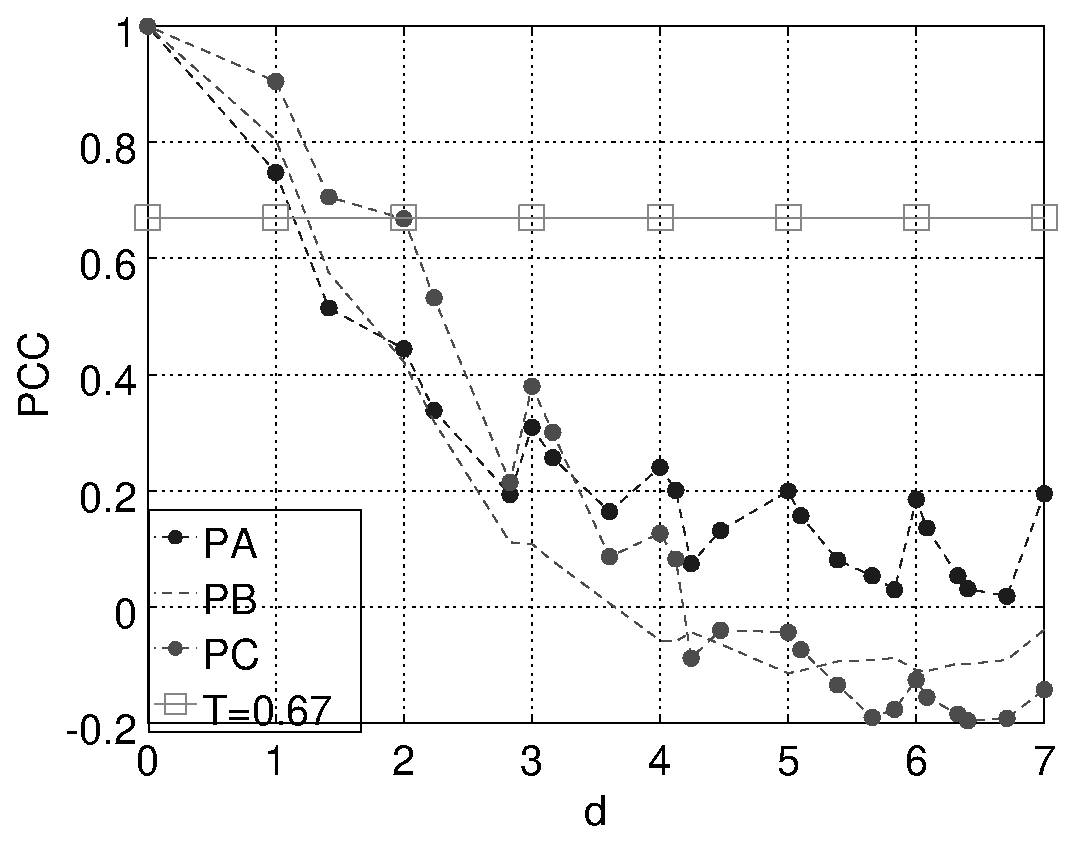
\includegraphics[width=.7\columnwidth]{image_plot-32zoom.eps}
  \caption{Region of analysis with a $WSIZE=32$ and a threshold of $0.67$.}
  \label{fig:choosingt32zoom}
\end{figure}
This means that the possibles used step length values
should be $l_0 \leq 2.8284$ pixels, given that
a superior value of $l_0$ cause correlation values smaller than $0.67$,
and this indicates by definition a lost analysis region.

Another example will be the case of the pattern $PA$, where $l_0\sqrt{2}/2 \leq 1.2$ pixels.
In these cases, we can only choose integers values to $l_0$, so that we choose
$l_0=1$ pixels.

\subsection{Choosing the search length}

The search length parameter ($L$), is the most free of the parameters.
In random patterns as $PA$ and $PC$ it only depends of computing power available.
In periodic patterns as $PB$, if the threshold is very low; by example,
with a threshold of $T=0.4$ in the Test-1 as in the Fig. \ref{fig:choosingt32}; the
value of $L$ should be $L \leq 9$ pixels. In other cases, $L$ can happen a false positive
in the recognition process of the analysis regions.

\subsection{Measure error in the PIV technique}
Like any measure technique, the $PIV$ technique also has considerations to 
estimate the maximum measure error in the calculus of the displacement.
To determinate analytically this data, we have to use the result of
Sec. \ref{subsec:steplength}, where was seen that the 
maximum (bi-dimensional) measure error, 
in predicting the displacement of an analysis region between two consecutive images,
is of $l_0\sqrt{2}/2$ pixels. Thus, given that in the process of $PIV$ technique 
we made $M-1$ comparison with the $M$ pictures, 
to determinate the maximum (possible) measure error $e$ in pixels, we use the next equation
\begin{equation}\label{eq:measureerror}
Measure~error\leq e\equiv l_0(M-1)\frac{\sqrt{2}}{2}
\end{equation}
For everything seen before, it's easy to notice that to get the maximum  measure error
in millimeters we use $l_0(M-1)\frac{\sqrt{2}}{2}~\beta$, where $\beta$ is the 
conversion factor of pixel to millimeters; thus, to improve $e$ we should
to minimize this relation, using pictures with a resolution 
as large as our computing power allows.

\section{NUMERICAL RESULTS}
The next figures show the result of submit a beam to a load and break static test;
thus, a system setup like the one described in the Sec. \ref{sec:systemdesc} was used.
The test results were captures using two methods,
the first method uses dial watches and the second apply the $PIV$ technique (see Sec. \ref{sec:algorithm}) over 
$M=19$ pictures, as described in the Sec. \ref{subsec:syssetup} following the procedure described
in the Algorithm \ref{alg:PIV}, with the consideration that in the pictures, $1$ pixel is
equivalent to $0.27027$ millimeters.

In the test, the  dial indicators will return the maximum deformation of the beam,
as it is shown in the Table \ref{tab:watch}. The Figs. \ref{fig:pivwindow} and  \ref{fig:system1}
describe the disposition of these indicators, where  the \textit{dial indicator 0}, \textit{dial indicator 1} 
and \textit{dial indicator 2} represent the indicators in the left, middle and the right, respectively.

\begin{table}[h]
  \begin{tabular}{ p{0.18\columnwidth} | p{0.18\columnwidth} | p{0.18\columnwidth} | p{0.18\columnwidth}}
    \hline
    ~                  & Dial indicator 0 & Dial indicator 1 & Dial indicator 2 \\ \hline \hline
   Maximum deformation & 6.75 mm & 11.29 mm & 6.9 mm \\ \hline
    
  \end{tabular}
  \caption{Beam deformation measure with the dial indicators. }
  \label{tab:watch}
\end{table}

On the other hand, using the $PIV$ technique, we select the analysis regions as showed in the
left image of Fig. \ref{fig:pivwindow}.   Dislocation
and rotation tests were apply over these analysis regions, 
as described in the Algs. \ref{alg:displacementtest} and \ref{alg:rotationtest},
respectively. The results of displacement tests can be seen in the 
Figs. \ref{fig:numresult1-des} and  \ref{fig:numresult1-des-max}.
It is easy to see in the Fig. \ref{fig:numresult1-des-max} 
that if there was only a displacement process over the analysis regions,
then it will be necessary to have a $l_0\sqrt{2}/2<2$ pixels ($l_0<2.8284$) 
to not exist a possibility of a false positive, in 
the recognition process, with a region located around of $17$ or $18$ pixels of neighborhood.
\begin{figure}[H]
\centering
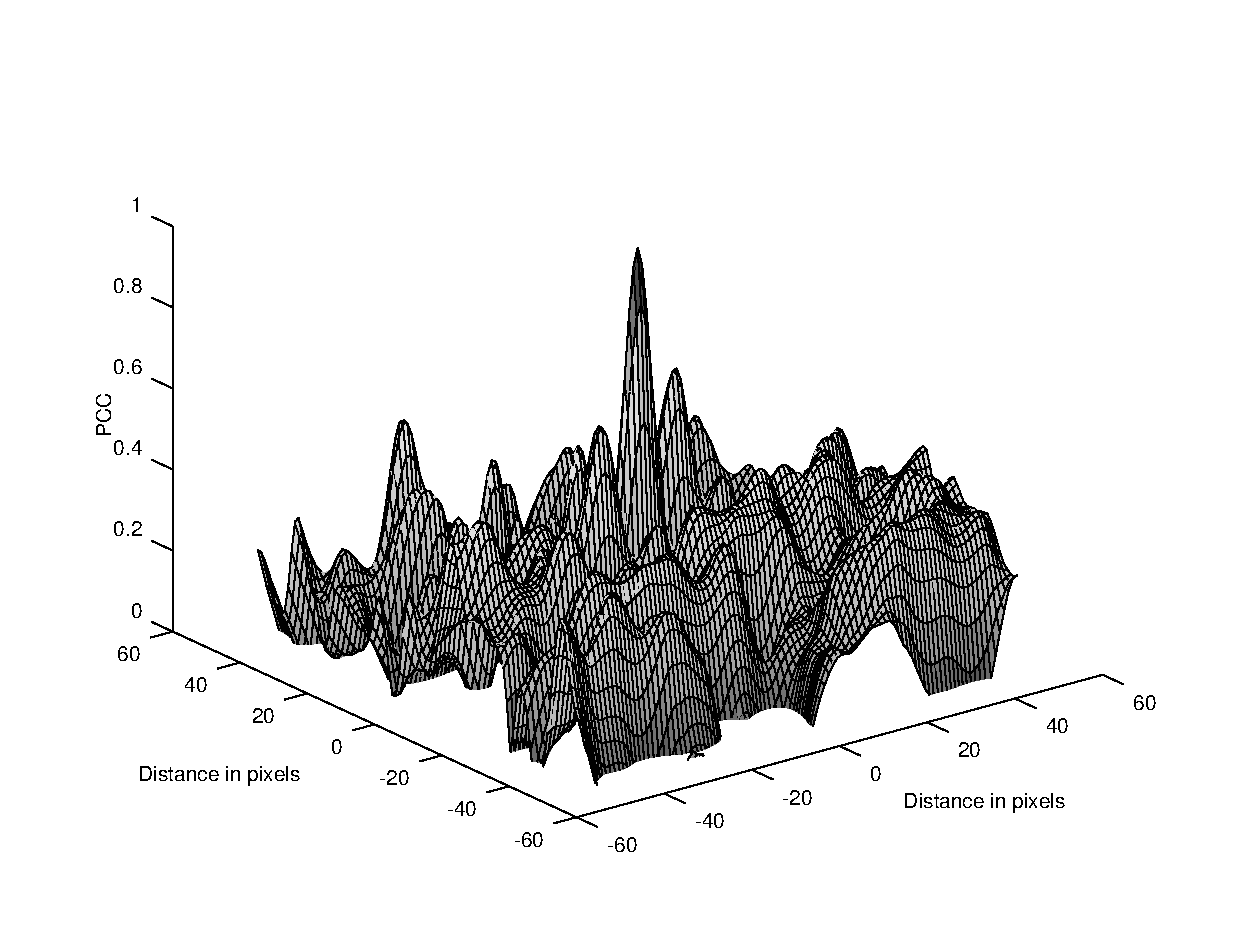
\includegraphics[width=\columnwidth]{PCC-Point0-multi_des.eps}
\caption{Displacement tests over the analysis region 0.}
\label{fig:numresult1-des}
\end{figure}
\begin{figure}[H]
\centering
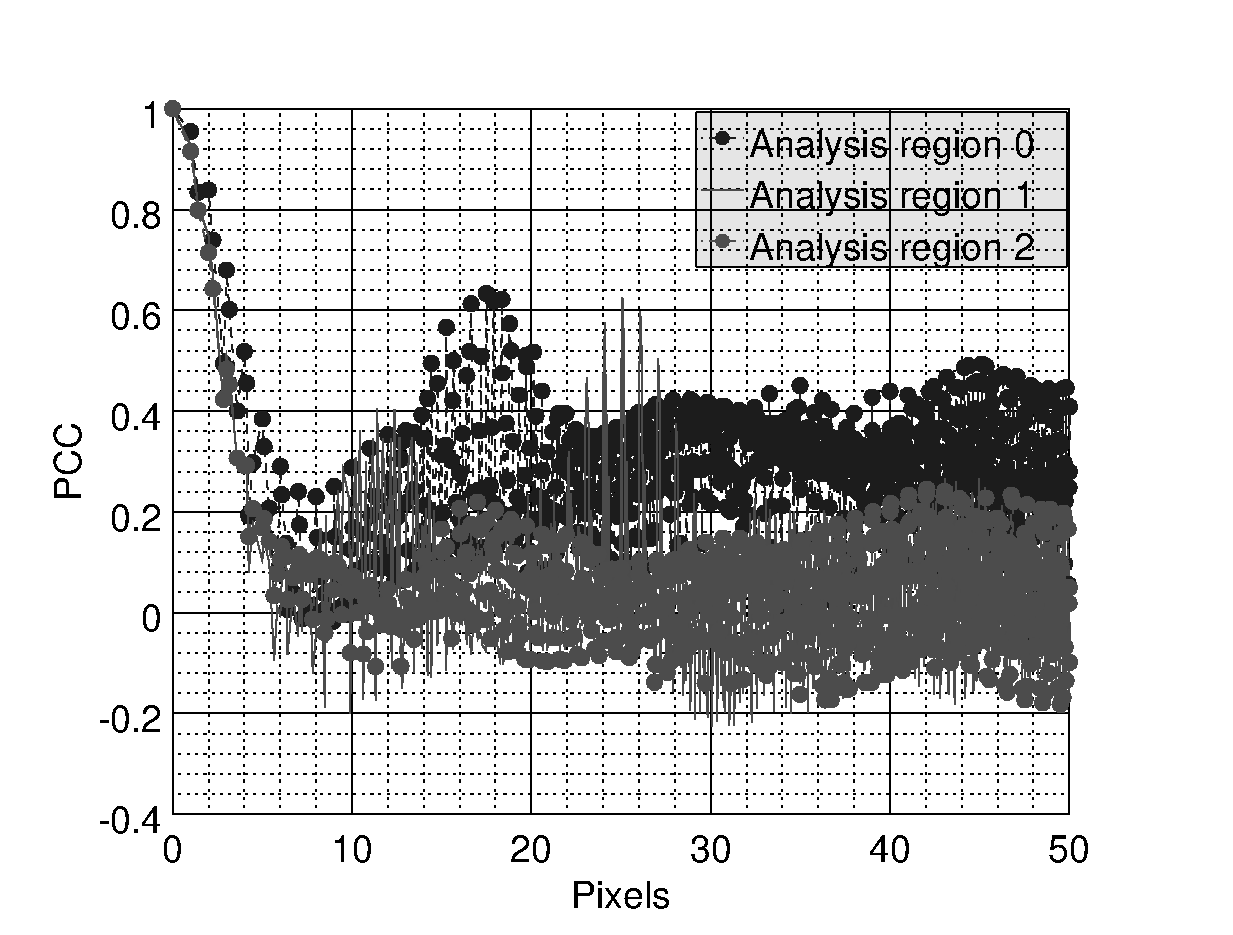
\includegraphics[width=\columnwidth]{numresult1-maketestjoint-multi_des_max.eps}
\caption{Displacement tests over the selected analysis regions showed in the radius form.}
\label{fig:numresult1-des-max}
\end{figure}

Additionally, the results of rotation test can be seen in the Fig. \ref{fig:numresult1-rot};
in this graphic it is easy to see that if there is only a rotation process over the 
analysis regions then on average the $PCC$ value decrease with the angle ($\alpha$ in degrees) 
following approximately the function $e^{-\left( \alpha/14\right)^2}$. Knowing that
the beam in last image has a horizontal rotation of $4.5^\circ$, then we can calculate that 
the mean rotation angle between the analysis region, of two consecutive images, 
is $0.25^\circ$, equivalent to a decrease of $PCC$ at $0.99972$.
\begin{figure}[H]
\centering
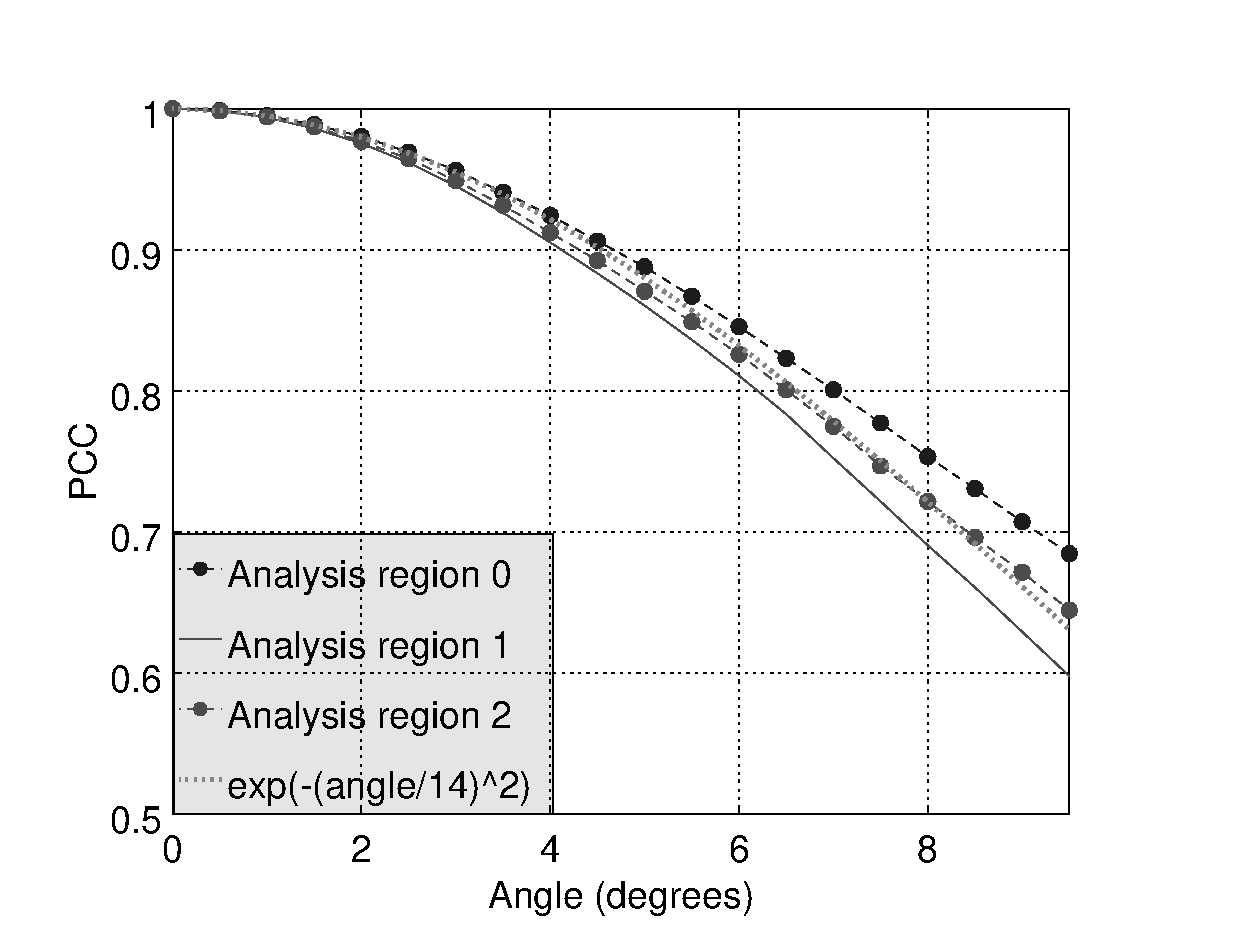
\includegraphics[width=\columnwidth]{numresult1-maketestjoint-rot.eps}
\caption{Rotation tests over the selected analysis regions.}
\label{fig:numresult1-rot}
\end{figure}
Thus, in the cases of analysis regions and pictures used, 
the procedure made between two images that most influence 
in the loss of correlation is the dislocation.


Using these results we can estimate that if we use the parameters:
$T=0.6$, $l_0=4$, $L=50$ and $WSIZE=32$, we are open to the possibility of introducing
error in the $PIV$ technique.
So that, for a $l_0=4$ the bi-dimensional measure error between images is at most $2.8284$ pixels 
(equivalent to $0.76444$ millimeters). Following the results in the 
Fig. \ref{fig:numresult1-des-max} for a measure error of $2.8284$ the $3$
analysis regions are located 
slightly above (analysis region 0), and 
slightly bellow (analysis regions 1 and 2) of the threshold $T=0.6$.
Thus, the analysis regions 1 and 2 are automatically discarded because they are below the threshold, 
furthermore the analysis region 0 is above the  threshold but has a $PCC$
value so close to a $PCC$ of a false positive located around of $17$ or $18$ pixels of neighborhood.
These considerations highlight that there will be errors in the results of $PIV$ 
algorithm, as it can be seen in the Fig. \ref{fig:numresult1testb} when compared to Table \ref{tab:watch}.

\begin{figure}[H]
\centering
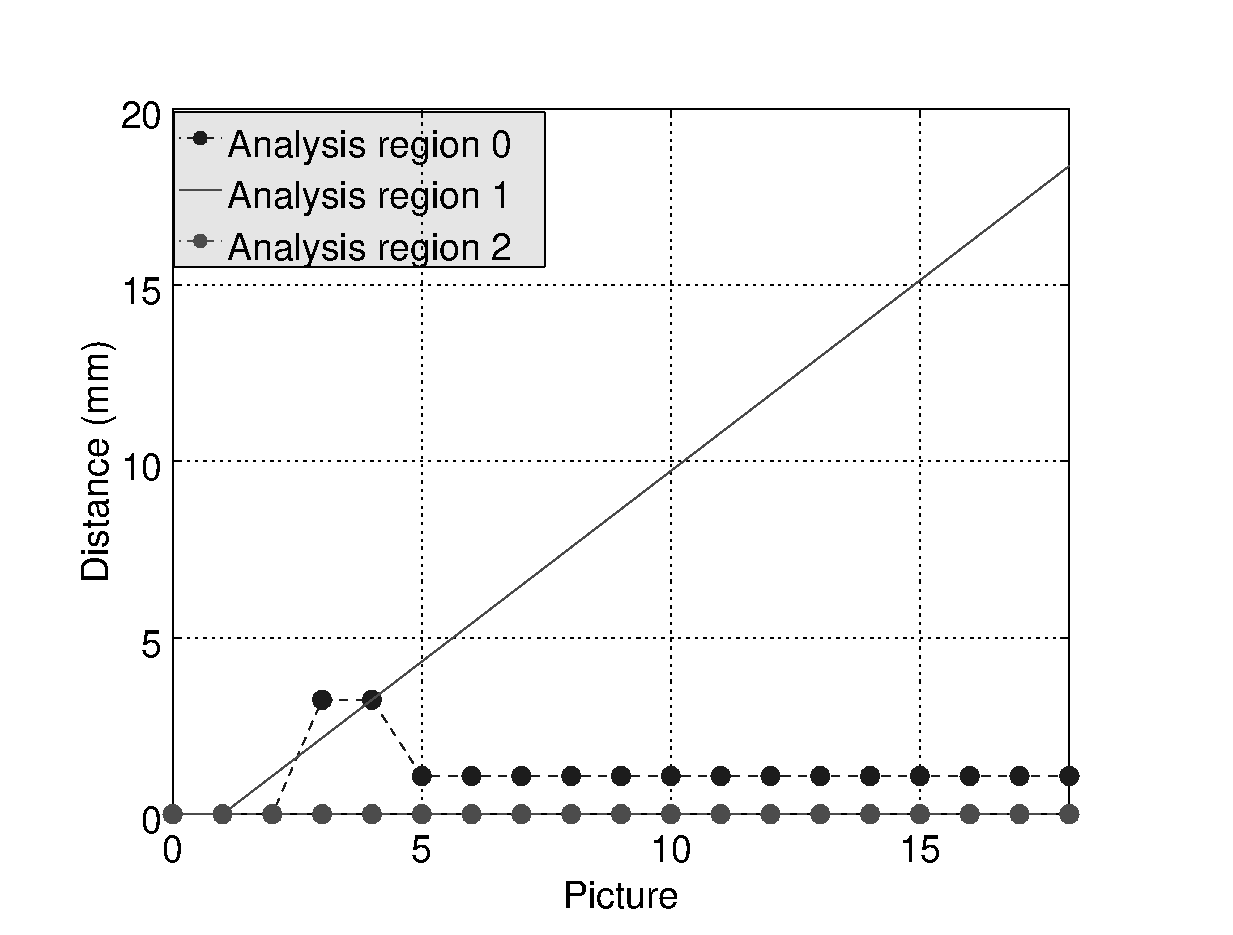
\includegraphics[width=\columnwidth]{numresult1-test-b.eps}
\caption{Tracking results of $PIV$ method over the selected analysis regions, with $l_0=4$ and $T=0.60$.}
\label{fig:numresult1testb}
\end{figure}


Moreover, we can estimate that if we use the parameters,
$T=0.82$, $l_0=1$, $L=50$ and $WSIZE=32$, we to get better results,
given that to a $l_0=1$ the bi-dimensional measure error is at most $0.70711$ pixels 
(equivalent to $0.19111$ millimeters).
Following the results in the Fig. \ref{fig:numresult1-des-max} 
to a measure error of $0.70711$ we can see that the $PCC$ value of the $3$
analysis regions are located much above of threshold $T=0.82$ and additionally
there is not the possibility of a false positive with any other group of pixels
because the unique pixels group that is above the threshold is the pixels group in a radius
of $0.70711$ pixels of origin.
Thus, with a measure error of $e=0.70711$ pixels across of $M=19$ images,
the maximum possible measure error in the $PIV$ technique will be $(M-1)e \equiv 12.728$ pixels
(in this case equivalent to $3.4400$ millimeters).
In the Fig. \ref{fig:numresult1testa} we can see th results of $PIV$ technique using these parameters,
if we compare these results to Table \ref{tab:watch} it is easy to see that the values are to close.
Table \ref{tab:watch2} presents this in detail, where are the maximum error is $0.60200 < 3.4400$ millimeters.
\begin{figure}[H]
\centering
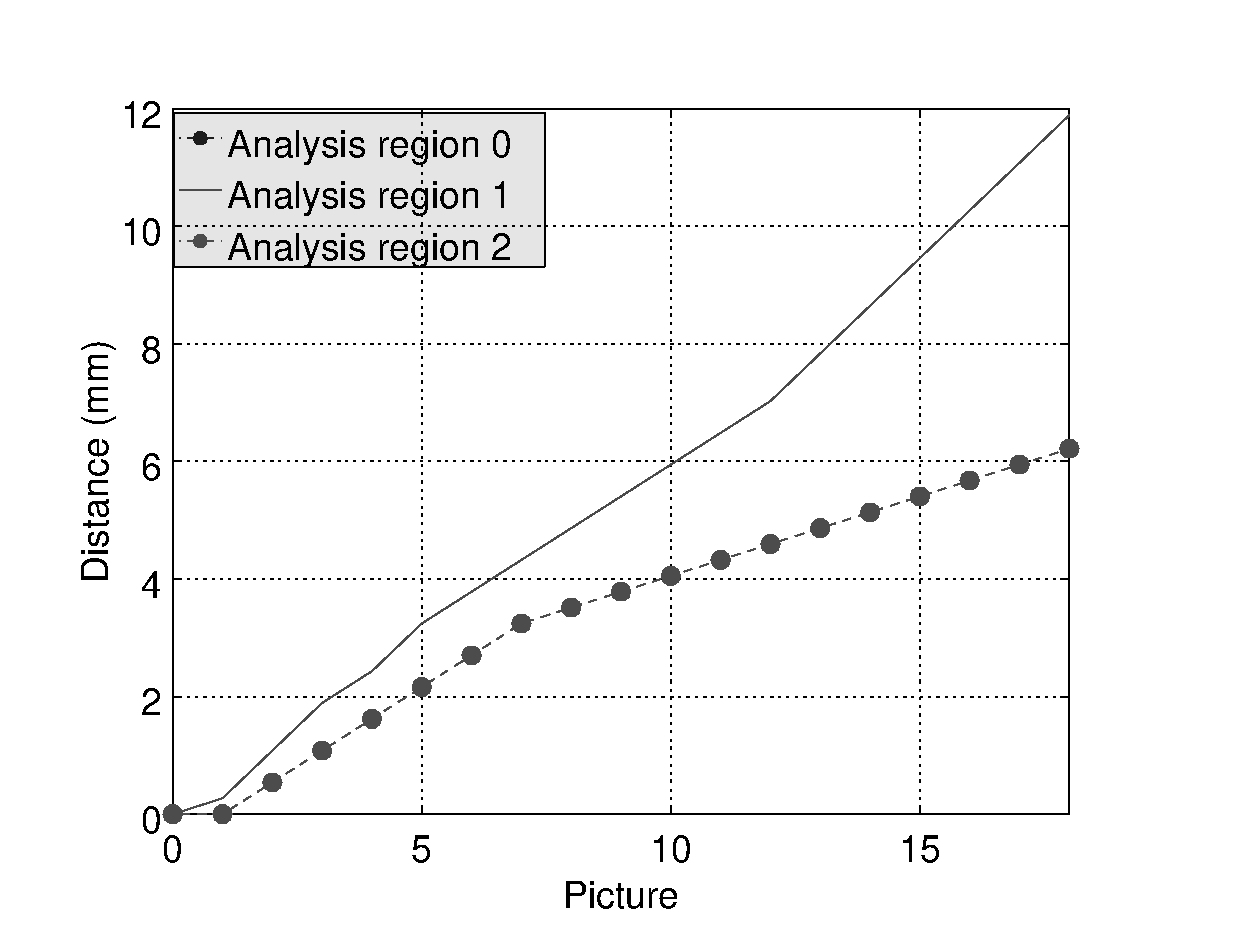
\includegraphics[width=\columnwidth]{numresult1-test-a.eps}
\caption{Tracking results of $PIV$ method over the selected analysis regions, with $l_0=1$ and $T=0.82$.}
\label{fig:numresult1testa}
\end{figure}

\begin{table}[h]
  \begin{tabular}{ p{0.18\columnwidth} | p{0.18\columnwidth} | p{0.18\columnwidth} | p{0.18\columnwidth}}
    \hline
    Error in      & Dial indicator 0 & Dial indicator 1 & Dial indicator 2 \\ \hline \hline
%    value & 6.2162 mm & 11.892 mm & 6.2162 mm \\ \hline
    millimeters & 0.5338 mm & 0.6020 mm & 0.6838 mm \\ \hline
    percentage  & 7.9081 \% & 5.3322 \% & 9.9101 \% \\ \hline
    
  \end{tabular}
  \caption{Error in the measure of beam deformation with the $PIV$ technique when compared with the dial indicators.}
  \label{tab:watch2}
\end{table}


%testes com diferentes parametros
% tabelas e graficos



\section{CONCLUSIONS}

Through the comparison of the traditional method 
to analyze load and break study of beams, using universal testing machine, 
to the technique using the particle image velocimetry method,
we observed similarity in the results when the adequate parameters criteria
to choose them were used.

The results shown in this paper demonstrated the importance of quality tests,
these are the displacement and rotation tests. Failure to observe these parameters
widens the possibility of false positives in the $PIV$ technique, and consequently
in the result of load and break study of beams.



\section*{ACKNOWLEDGMENT}

We wish to acknowledge the partial financial support for this study provided by the $CAPES$ scholarship
$PNPD$ Program.

\section{APPENDIX: ALGORITHM DESCRIPTION} 
\label{sec:algorithm}

The Algorithm \ref{alg:PIV} shows the procedure of $PIV$ method implemented in this work.
The algorithm needs as input data a set of $M$ pictures $P_m$, for all
$m$ integer so that  $0 \leq m \leq M-1$. 
These pictures represent the process of load and break static test; for 
this purpose, in the picture $P_0$, $N$ points $X_0^n$, for all
$n$ integer so that  $0 \leq n \leq N-1$ will be chosen.
Thus, the algorithm tracks these $N$ points through the $M$ images $P_m$

%%%%%%%%%%%%%%%%%%%%%%%%%%%%%%%%%%%%%%%%%%%%%%%%%%%%%%%%%%%%%%%%%%%%%
%%%%%%%%%%%%%%%%%%%%%%%%%%%%%%%%%%%%%%%%%%%%%%%%%%%%%%%%%%%%%%%%%%%%%
\begin{algorithm}[!h]
\SetKwInOut{Variables}{Variables}

 \KwData{A set of $M$ pictures $P_m$ taken each $\tau$ seconds.}
 \KwResult{$X_{m}^n$, a path that describe the deformation of the beam 
 caused by load and break study of $N$ analysis regions across $M$ Pictures.}

 ~\\
 $\{X_0^n,WSIZE\} \leftarrow$ quality\_test($P_0$)\;
 ~\\
 Choose the values of $\tau$, $l_0$ and $L$\;
 ~\\
 \For{$m\leftarrow 1$ \KwTo $M-1$ }{
  \For{$n\leftarrow 0$ \KwTo $N-1$ }{
  $\{X_{m}^n,Found\}$ $\leftarrow$ search\_arround\_of($X_{m-1}^n$,$A_{m-1}^n$,$P_m$)
  
  }
 }
\caption{PIV algorithm}
\label{alg:PIV} 
\end{algorithm}
The function $quality\_test()$, described in the Algorithm \ref{alg:qualitytest}, 
helps the user to choose
the better position of initial tracking points $X_{0}^n$, in the picture
$P_0$, and the side size ($WSIZE$) of the analysis regions $A_{0}^n$.
This function uses internally the functions 
$make\_displacemente\_test()$ and 
$make\_rotation\_test()$, that are described in the Algorithm \ref{alg:displacementtest}
and \ref{alg:rotationtest}, respectively. Section \ref{sec:qualitytests}
shows some examples of a quality test.


%%%%%%%%%%%%%%%%%%%%%%%%%%%%%%%%%%%%%%%%%%%%%%%%%%%%%%%%%%%%%%%%%%%%%
%%%%%%%%%%%%%%%%%%%%%%%%%%%%%%%%%%%%%%%%%%%%%%%%%%%%%%%%%%%%%%%%%%%%%
\begin{algorithm}[!h]
\SetKwInOut{Input}{Input}
\SetKwInOut{Output}{Output}

\SetKwProg{Fn}{Function}{ is}{end}
\Fn{  quality\_test($P$)}{
  \Input{It use a picture $P$ where will be chosen a set of $N$ initial analysis region.}
  \Output{$\{X^n,WSIZE\}$, the points $X^n$ where the analysis regions  and 
  a variable $WSIZE$ that indicates their side size will be chosen.}
  \Repeat{User approves the results of displacement and rotation tests}
  {
    $\bullet$ Choose the values of $N$ and $WSIZE$\; 
    $\bullet$ Select $N$ points $X^n$ in the picture $P$\;
    $\bullet$ Conform in $X^n$ and over $P$ a set of analysis 
    regions $A^n$ of side $WSIZE$ pixels\;
    \For{$n\leftarrow 0$ \KwTo $N-1$}{
      make\_displacement\_test($X^n$,$WSIZE$,$P$)\;
      make\_rotation\_test($X^n$,$WSIZE$,$P$)\;
    }
  }
}
\caption{Quality test of chosen points.}
\label{alg:qualitytest} 
\end{algorithm}

The Algorithm \ref{alg:displacementtest} returns a graphic where a curve
that describe the $PCC$ value between an
initial analysis region in $(i_0,j_0)$ and its neighbors in $(i,j)$ that fulfill 
$0 \leq |i-i_0|< d_{max}$ and $0 \leq |j-j_0| < d_{max}$.
Here we suggest that $d_{max}\equiv L$.
%%%%%%%%%%%%%%%%%%%%%%%%%%%%%%%%%%%%%%%%%%%%%%%%%%%%%%%%%%%%%%%%%%%%%
%%%%%%%%%%%%%%%%%%%%%%%%%%%%%%%%%%%%%%%%%%%%%%%%%%%%%%%%%%%%%%%%%%%%%
\begin{algorithm}[!h]
\SetKwInOut{Input}{Input}
\SetKwInOut{Output}{Output}

\SetKwProg{Fn}{Function}{ is}{end}
\Fn{  make\_displacement\_test($X$,$WSIZE$,$P$)}{
  \Input{A picture $P$, a point $X\equiv (i_0,j_0)$ and a variable $WSIZE$.}
  \Output{A figure with the correlation of an analysis region, in 
  the point $X$, with your neighbor analysis regions.}
 ~\\
  Conform in $X$ and over $P$ an analysis region $A_0$ of side $WSIZE$ pixels\;
 ~\\  
  Choose the value $d_{max}>0$\;
 ~\\  
  \For{$a \leftarrow -(d_{max}-1)$ \KwTo $d_{max}-1$ }{
    \For{$b \leftarrow -(d_{max}-1)$ \KwTo $d_{max}-1$ }{
      $X_{ab} \leftarrow X + (a,b)$\;
      Conform in  $P$ and around the central point $X_{ab}$  an analysis region $A_{ab}$ of side $WSIZE$ pixels\;
      $C_{ab} \leftarrow \rho(A_0,A_{ab})$
    }
  }
  
  Plot the values of $C_{ab}$\;
 ~\\  
  Plot $C_{d}$ from $C_{ab}$, so that $d=\sqrt{a^2+b^2}$ $\forall$ $-(d_{max}-1)\leq a,b \leq d_{max}-1$, and using
  the highest value of $PCC$ when many $PCC$ values coincide with the same distance $d$\; 
}
\caption{Displacement test of one point.}
\label{alg:displacementtest} 
\end{algorithm}

The Algorithm \ref{alg:rotationtest} returns a graphic where
is showed a curve that describe the $PCC$ value between an
analysis region a your rotated versions until a angle $\alpha_{max}$ degrees.
%%%%%%%%%%%%%%%%%%%%%%%%%%%%%%%%%%%%%%%%%%%%%%%%%%%%%%%%%%%%%%%%%%%%%
%%%%%%%%%%%%%%%%%%%%%%%%%%%%%%%%%%%%%%%%%%%%%%%%%%%%%%%%%%%%%%%%%%%%%
\begin{algorithm}[!h]
\SetKwInOut{Input}{Input}
\SetKwInOut{Output}{Output}

\SetKwProg{Fn}{Function}{ is}{end}
\Fn{  make\_rotation\_test($X$,$WSIZE$,$P$)}{
  \Input{A picture $P$, a point $X\equiv (i_0,j_0)$ and a variable $WSIZE$.}
  \Output{A figure with the correlation of an analysis region, in 
  the point $X$, with its rotated versions.}

  Conform in $P$ and around the point $X$ an analysis region $B_0$ of side $WSIZE$ pixels\;
  Choose the value $\alpha_{max}>0$ degrees\;
  
  \For{$i \leftarrow 0$ \KwTo $\lfloor\alpha_{max}/0.5\rfloor$ }{
    $\alpha_i \leftarrow 0.5 i$\;
    Conform in $P$ and around the point $X$ an analysis region $B_i$ of side $WSIZE$ pixels
    rotated an angle $\alpha_i$\;
    $C_i \leftarrow \rho(B_0,B_i)$
  }
  
  Plot the values of $C_i$ versus $\alpha_i$.
}
\caption{Rotation test of one point.}
\label{alg:rotationtest} 
\end{algorithm}

In the Algorithm \ref{alg:PIV}  the variables $L$, $l_0$ and $\tau$, were also chosen.
The criteria to select these values using the results of quality test
can be seen in the Sec. \ref{sec:criteria}.
By other side, in the Algorithm \ref{alg:PIV}, the function $search\_arround\_of()$, 
described in the Algorithm \ref{alg:SearchArround}, searches for
an analysis region that matches $A_{m-1}^n$, around the point $X_{m-1}^n$ 
in the picture $P_m$, and, if the match exists, then the
point $X_{m}^n$ of match is returned, joint with the variable $Found$ loaded with $True$; in other cases
$Found$ is loaded with $False$. 

%%%%%%%%%%%%%%%%%%%%%%%%%%%%%%%%%%%%%%%%%%%%%%%%%%%%%%%%%%%%%%%%%%%%%
%%%%%%%%%%%%%%%%%%%%%%%%%%%%%%%%%%%%%%%%%%%%%%%%%%%%%%%%%%%%%%%%%%%%%
\begin{algorithm}[!h]
\SetKwInOut{Input}{Input}
\SetKwInOut{Output}{Output}

\SetKwProg{Fn}{Function}{ is}{end}
\Fn{  search\_arround\_of($X$,$A$,$P$)}{
  \Input{It use a picture $P$ where an analysis region 
  that match with $A$ will be searched, this region will be searched around the $X$ point.}
  \Output{$\{Y,Found\}$, the point $Y$ where a match with $A$ and 
  a variable $Found$ that indicates if the match exist are found.}
\begin{flalign*}
 Found & \leftarrow False & \\
 Y &\leftarrow X & \\
 OldPCC & \leftarrow -1.0 & \\
 i & \leftarrow 0 & \\
 j & \leftarrow 0 & %
\end{flalign*}

  \While{$l_0 i\leq L$ }{
  \While{$l_0 j\leq L$ }{
  
   $\bullet$ $y \leftarrow X+(l_0~ i,l_0~j)$\;
   $\bullet$ Conform in $P$ and around the point $y$ an analysis region $R$ of side $WSIZE$ pixels\;
   $\bullet$ $PCC \leftarrow \rho(R,A)$\;
   ~\\
   
    \If{$PCC\geq T$ \textbf{and} $PCC \geq OldPCC$ }{
      \begin{flalign*}
      Y & \leftarrow y & \\
      Found & \leftarrow True & \\
      OldPCC & \leftarrow PCC & %
      \end{flalign*}
    }
    $i\leftarrow i+1$\;$j\leftarrow j+1$\;
  }
  }
}
\caption{Search a match with $A$, around a point $X$ in a picture $P$.}
\label{alg:SearchArround} 
\end{algorithm}





%FAPEMIG\\
%numero de bolsa\\
%numero de projeto\\
%numero de aluno


\bibliography{article}   %>>>> bibliography data in report.bib
\bibliographystyle{apalike}

\end{document}

